\documentclass[a4paper, 12pt]{report}
\usepackage[utf8]{inputenc}
\usepackage[bookmarks, breaklinks, colorlinks]{hyperref}
\hypersetup{
	citecolor=black,
	linkcolor=black,
	filecolor=black,
	urlcolor=black
}

\usepackage{graphicx}
\usepackage{pdfpages}
\usepackage{tocbibind}

% Packages and configuration for Alloy code listing
\usepackage{listings}
\usepackage{alloy}
\usepackage{color}
\definecolor{alloy-keyword}{rgb}{0.23, 0.23, 0.7}
\definecolor{alloy-comment}{rgb}{0.18, 0.64, 0.18}
\definecolor{alloy-string}{rgb}{0.71, 0.18, 0.71}

\def\chapterautorefname{Chapter}


\title{
	\begin{figure}[h]
		\centering
		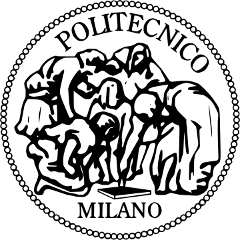
\includegraphics{../common_resources/logo_polimi.png}
	\end{figure}
	\vspace{30px}
	Software Engineering 2 Project: PowerEnJoy \\ \vspace{1em}
	\textbf{R}equirements \textbf{A}nalysis and \textbf{S}pecification \textbf{D}ocument
}
	

\author{Marco Ieni, Francesco Lamonaca, Marco Miglionico\\Politecnico di Milano, A.A. 2016/2017}
\date{\today\\v1.0}

\begin{document}
\maketitle
\tableofcontents
% \listoffigures
% \listoftables

\chapter{Introduction}
\label{ch:introduction}
\section{Purpose}
This is the Design Document of PowerEnJoy, a digital management system for a car-sharing service that exclusively employs electric cars.
The aim of this document is to show our design choices and the rationale behind them. 

We will analyse the component of the system and how they interact between each other.
Furthermore, we will show the most important algorithms of the project, in order to underline the key aspects of their implementation.
Finally, we will add details to the first description of the user interfaces that was described in the RASD.

\section{Scope}

\section{Definitions, acronyms, abbreviations}
\begin{description}
    \item[JPA:] The Java Persistence API (JPA) is a Java application programming interface specification that describes the management of relational data.
    \item[RASD:] Requirements Analysis and Specification Document.
\end{description}

\section{Reference Documents}
This document refers to the project rules of the Software Engineering 2
project, to the template for the Design Document contained into it and to Requirement Analysis and Specification Document (the previous delivered document)

\section{Overview}
In this section we will present the high level components of the system and their interaction:

\begin{description}
\item[Mobile application:] This presentation layer consists in the mobile client. It communicates directly with the application server.
\item[Application Server:] This layer contains all the application logic of the system. All the policies, the algorithms and the computation are performed here. This layer offers a service-oriented interface.
\item[Database:] The data layer is responsible for the data storage and retrieval. It does not implement any application logic. This layer must guarantee ACID properties. 
\end{description}

\begin{figure}
	\centering
	\includegraphics[scale=0.6]{architectural_design/Architecture_Diagrams/Layers.png}
	\caption{Layers of the system.}
	\label{fig:layers}
\end{figure}

The system is structured in three layers as we can see in picture \ref{fig:layers}.

This design choice makes it possible to deploy the application server and the database on different tiers. It also improves scalability and fault tolerance.

\begin{figure}
	\centering
	\includegraphics[scale=0.6]{architectural_design/Architecture_Diagrams/Tier.png}
	\caption{Tiers of the system.}
	\label{fig:tiers}
\end{figure}

The figure \ref{fig:tiers}, instead, shows the three tiers from a very high level point of view.

\begin{figure}
	\centering
	\includegraphics[width=\textwidth,height=\dimexpr\textheight-4\baselineskip-\abovecaptionskip-\belowcaptionskip\relax,keepaspectratio]{architectural_design/Architecture_Diagrams/Tier2.png}
	\caption{High level components of the system.}
	\label{fig:high_components}
\end{figure}

The interactions between the main components are shown in the figure \ref{fig:high_components}.

\begin{figure}
    \vspace*{-2cm}
    \makebox[\linewidth]{
        \includegraphics[width=1.3\linewidth]{architectural_design/Architecture_Diagrams/Tier3.png}
    }
    \caption{Description of the tiers, detailed with Java EE components.}
	\label{fig:tiers_description}
\end{figure}

A more detailed description of the three different tiers is shown in picture \ref{fig:tiers_description}.



\section{Goals}
The goals of the PowerEnJoy software are the following:
\begin{enumerate}
	\item allows the user to book a car for up to an hour before he/she pick it up;
	\item allows the user to login to the service;  
	\item allows the user to search for a car in a specific location; 
	\item allows the user to find the closest cars with respect to his/her position; 
	\item allows the user to know in every moment the current fee he/she has to pay;
	\item allows the user to park in specific areas called safe areas;
	\item allows the user to unlock the vehicle when he/she is next to it using the mobile app;
	\item allows the user to obtain a 10\% discount if he/she takes at least 2 passengers;
	\item allows the user to recharge a car only in a power grid station;
	\item allows the user to obtain a 20\% discount if the car is left with no more than 50\% of battery empty;
	\item allows the user to obtain a 30\% discount if the car is left in a special parking area in which they can be recharged and the user takes care of plugging the car into the power grid;
	\item the system charge the user 30\% on the last ride if the car is left at more than 3 KM from the nearest power grid station;
	\item the system charge the user 30\% on the last ride if the car is left with more than 80\% of the battery empty;
	\item allows the user to enable the saving mode option;
	\item allows the user to enable the parking mode option;
	
	
\end{enumerate}
\section{Constraints}
%Anything that will limit the developer’s options (e.g. regulations, reliability, criticality, hardware limitations, parallelism, law, etc)
\begin{description}
\item[Regulatory policies:] It is user responsibility to ensure that the use of the system complies with the
local laws and policies.
The system must ask the user for the permission to acquire, store and process personal data. Furthermore, the system must offer to the user the possibility to delete all the personal data.
\item[Hardware limitations:] PowerEnJoy application will require a device with Android 4.0.3+ or IOS 8+ to work. In addition to this, the device must have access to the Internet and the GPS must be enabled when the user wants to unlock the car or when he wants to do a research of a car based on their position.
\item[Reliability requirements:] The system must have a minimum availability of 99.9\%.
\item[Safety and security considerations:] All the data about the user, including their position and routes, must be kept private.
Therefore, these data must not be accessible from external subjects (e.g. advertising agencies).
\end{description}

\section{Stakeholders}
The only stakeholder is the company that commissioned the project. They want the right compromise between initial and maintenance cost, usability, efficiency, effectiveness, reliability and robustness.
% Effectiveness: The extent to which the software satisfies the user and meets user requirements.
% Reliability: How reliable the software is in performing required functions under different scenarios/conditions.
% Robustness – How robust the software is under unexpected events like software crash, power-off etc and saves its data.
\section{Actors}
The actors of our system are the visitors and the users.

\subsection{Visitor}
The visitor is a person who is not logged in to the system. The functionalities that he/she is able to do are sign up and login.

In order to register to PowerEnJoy service, the visitor must provide the following data:
\begin{itemize}
	\item name
	\item surname
	\item e-mail address
	\item date of birth
	\item sex
	\item country of birth
	\item phone number
	\item province of birth
	\item tax id code % English for Italian "codice fiscale"
	\item document information, that has to be validated
	\item residential address
	\item living address
	\item patent number, that has to be validated from the motorization;
	\item payment information;
\end{itemize}

The phone number is accepted as it is, the e-mail address must be validated with a token and all
the other data must be validated by the proper authorities.

\subsection{User}
The user is a person who logged in to the system. He has access to the following functionalities:
\begin{itemize}
	\item book a car
	\item ...
\end{itemize}

\subsection{Driver}
The driver is a special case user that opened the car and inserted is password in the screen. He has access to the following functionalities:
\begin{itemize}
	\item money saving option (insert destination and receive nearest power grid station)
	\item park the car in a safe area
\end{itemize}

\chapter{Overall Description}
\label{ch:overall_description}
\section{Product prespective}
% Describes external interfaces: system, user, hardware, software; also operations and site adaptation, and hardware constraints.
% It defines the boundaries of the system. Further details on the shared phenomena and a domain model (class diagrams, and statecharts)

The PowerEnJoy front end is only composed of a mobile app.
%There can be a website that contains only information and reminds to the link of the app in both Apple Store and Play Store, but it is not our purpose to develop it.
The system developed will not be integrated with other existing systems that managed a car-sharing service.

Also, the system will only be user based, this means no internal interface will be developed for now.
For example, it will be possible to modify the safe areas and the power grid stations only by the database interface, so editing the tables directly.
In the future some API will be provided, in order to permit the evolution of the features of the system.

The interaction with the car is managed by "HandyCar", a system that abstract all the operations related to the interaction with the car, like lock and unlock the car, know his battery level, the number of passengers and so on.


\subsection{User Interfaces}
All the interfaces shall be intuitive and user friendly and they should not
require the reading of detailed documentation to be used.

Below are presented the mockup of the main screens of the Android mobile app version, in order to give an idea of the final product.

\subsubsection*{Login}

\begin{figure}
	\centering
	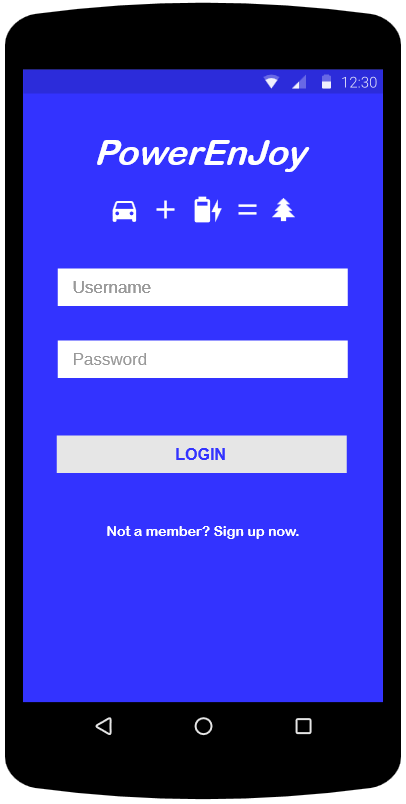
\includegraphics[width=\textwidth,height=\dimexpr\textheight-4\baselineskip-\abovecaptionskip-\belowcaptionskip\relax,keepaspectratio]{overall_description/mockup/login.png}
	\caption{Login and registration page.}
	\label{fig:mockup_login}
\end{figure}

When the user open the mobile app for the first time he/she will visualize the login screen, which is reported in figure \ref{fig:mockup_login}. Here the user can insert his/her username and password couple if he/she has one, otherwise he/she can register to the service. When the user does the login he/she will visualize the Main page.

\subsubsection*{Main page}

\begin{figure}
	\centering
	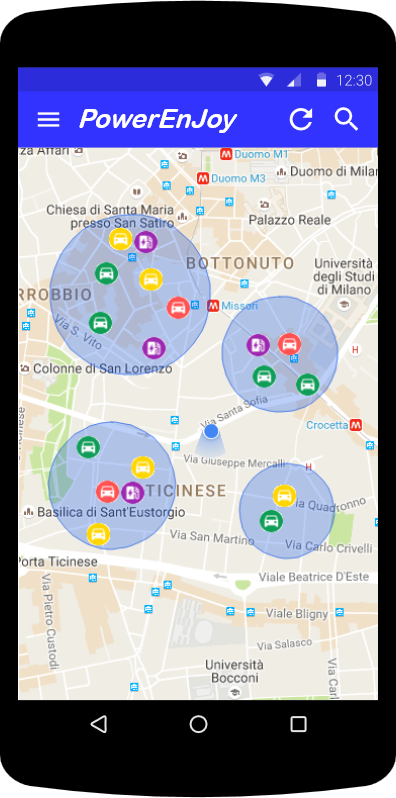
\includegraphics[width=\textwidth,height=\dimexpr\textheight-4\baselineskip-\abovecaptionskip-\belowcaptionskip\relax,keepaspectratio]{overall_description/mockup/main_page.png}
	\caption{Main page.}
	\label{fig:mockup_main_page}
\end{figure}

In figure \ref{fig:mockup_main_page} is represented the first page that is shown to the user if it logged in to the system before.

From this page a user can search for the nearest available car having a quick look to their battery level, too.

The legend of the battery level is the following:
\begin{description}
	\item[red:] battery level from 1\% to 19\%;
	\item[yellow:] battery level from 20\% to 49\%;
	\item[green:] battery level from 50\% to 100\%.
\end{description}

\subsubsection*{Car selection}

\begin{figure}
	\centering
	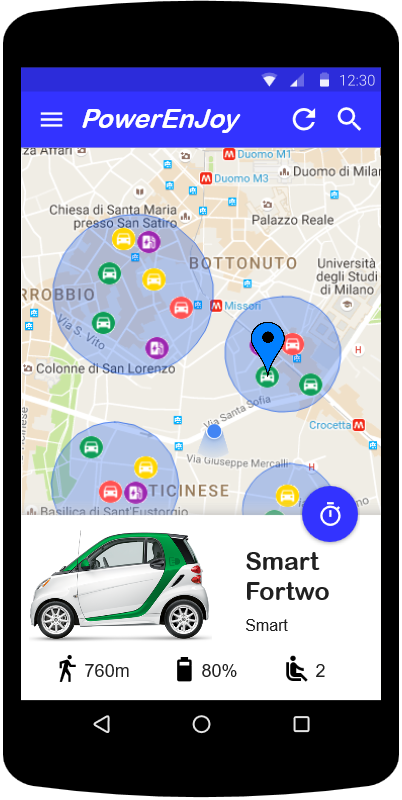
\includegraphics[width=\textwidth,height=\dimexpr\textheight-4\baselineskip-\abovecaptionskip-\belowcaptionskip\relax,keepaspectratio]{overall_description/mockup/car_selection.png}
	\caption{Car selection.}
	\label{fig:mockup_car_selection}
\end{figure}

From the Main page, when the user selects a car a bottom sheets slides up from the bottom of the screen to reveal the car information and a marker will appear over the car that he/she selected. You can reserve the car by clicking on the blue bottom with the timer icon (a yes/no confirmation will appear). You can see this screen in figure \ref{fig:mockup_car_selection}.

\subsubsection*{Car unlock}

\begin{figure}
	\centering
	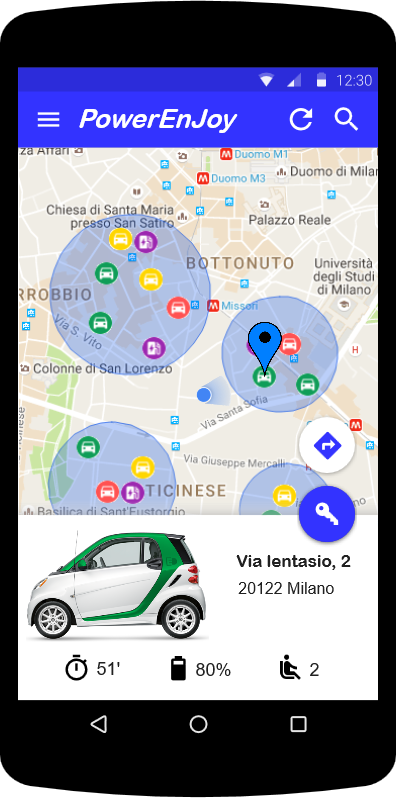
\includegraphics[width=\textwidth,height=\dimexpr\textheight-4\baselineskip-\abovecaptionskip-\belowcaptionskip\relax,keepaspectratio]{overall_description/mockup/car_unlock.png}
	\caption{Car unlock.}
	\label{fig:mockup_car_unlock}
\end{figure}

After the reservation of the car, you can see how the screen changes in figure \ref{fig:mockup_car_unlock}. The user can find indications to the car by pressing the white button that appears and when he/she is near to the car he/she can press the button with the key.

\subsection{Hardware interfaces}
In the system there are the following hardware interfaces:
\begin{description}
	\item [Panic button:] a button that is present in every car and can be pressed by the user to report that there something wrong with the mechanical aspects of the car;
	\item [GPS:] it's used to track the position of cars and users;
	\item [HandyCar Board:] a board to which all the actuators and sensors of the car are connected. The sensors system that detects how many passengers there are in the car it's connected to this board too, so the board can memorize the maximum number of passengers of the current ride.
\end{description}

\subsection{Software interfaces}
The mobile app will be developed both for IOS and Android, so the system will use the API of these operating systems to access to the GPS of the smartphone and maps.

Furthermore, the HandyCar Board provides some simple API, in order to control the board remotely through the Internet.

The other software interfaces that we have are the external payment	gateway and the motorization gateway.





\section{Product Functions}
%Summary of major functions. It's a sort of summary of the requirements. 
Product Functions.
\begin{description}
\item[Sign up:] a visitor registers to PowerEnJoy service providing the following data:
	\begin{itemize}
	\item name;
	\item surname;
	\item e-mail address;
	\item date of birth;
	\item sex;
	\item country of birth;
	\item phone number;
	\item province of birth;
	\item tax id code; % English for Italian "codice fiscale"
	\item document information, that has to be validated;
	\item residential address;
	\item living address;
	\item payment information.
	\end{itemize}
	The user will receive back a password that can be used to access the system.
\item[Login:] a user accesses the system using the e-mail address they provided in the registration and the password they received.
\item[Edit profile data:] a user deletes their data, to keep them updated for example.
\item[Delete account:] a user deletes his account.
\item[Look for a car with user position:] a user look for a car basing the research on their devices position.
\item[Look for a car with a specified address:] a user look for a car basing the research on a specific address.
\item[Reserve a car:] a user book a car that he found in a previous research. He has one hour of time to reach the car and unlock it, otherwise the reservation expires and he has to pay a fee of 1 EUR.
%I am not sure if to include "unlock a car" and "start the car" in this section
\item[Unlock a car:] a user unlocks a car that he previously reserved at maximum one hour before. This option will be available to the user only if the GPS of his device is recognized at maximum at 6 meter from the car.
\item[Start the car:] a user that has unlocked the car starts the engine of the car by inserting his password in the tablet of the car
\item[Know the current fee:] a user looks at the tablet of the car and reads the current fee. He can do this in every moment when he is in the vehicle, because the current fee is always displayed.
\item[Recharge the car:] a user connects the car to a plug of a power grid station.
\item[Enable saving money option:] a user enables the money saving option by clicking on the corresponding button in the tablet interface. At this point, he/she can input his/her final destination and the system provides information about the station where to leave the car to get a discount.
This station is determined to ensure a uniform distribution of cars in the city and depends both on the destination of the user and on the availability of power plugs at the selected station. 
\item[End the ride:] the system stops charging the user as soon as the car is parked in a safe area and the user 
exits the car.
\end{description}

\section{User Characteristics}
User needs to have a device with Android or IOS with the PowerEnJoy app installed on it.
In addition, the device needs to have access to Internet and the GPS enabled.

PowerEnJoy aims to reach any person who needs to share a car, regardless his cultural or instruction level, so everyone with a basic knowledge of mobile applications will be able to access easily the service.

The user has to be registered and logged into the system in to the system in order to access his functions.

\section{Constraints}
%Anything that will limit the developer’s options (e.g. regulations, reliability, criticality, hardware limitations, parallelism, law, etc)
\begin{description}
\item[Regulatory policies:] It is user responsibility to ensure that the use of the system complies with the
local laws and policies.
The system must ask the user for the permission to acquire, store and process personal data. Furthermore, the system must offer to the user the possibility to delete all the personal data.
\item[Hardware limitations:] PowerEnJoy application will require a device with Android 4.0.3+ or IOS 8+ to work. In addition to this, the device must have access to the Internet and the GPS must be enabled when the user wants to unlock the car or when he wants to do a research of a car based on their position.
\item[Reliability requirements:] The system must have a minimum availability of 99.9\%.
\item[Safety and security considerations:] All the data about the user, including their position and routes, must be kept private.
Therefore, these data must not be accessible from external subjects (e.g. advertising agencies).
\end{description}

\section{Assumption and Dependencies}

\subsection{Text Assumptions}
\begin{enumerate}
	\item the mobile application can work also without GPS enabled because the user can manually insert the address of the starting point;
	\item the system track the position of the cars and of the users;
	\item we assume that the validity of the driving license are checked by an external system;
	\item the payments are handled by an external system;
	\item the car has a tablet that display the current bill the user has to pay;
	\item when a car is parked in a power grid station the user can start plugging the car within 10 minutes and during this time the company won't plug it;
	\item the discounts are cumulative
	\item the unusable (without battery) or almost unusable cars that are not in a power grid station or that can't reach a power station with the current battery will be charge on site by the maintainers of the company;
	\item the user is able to search for a car within a range of 1 km from his/her position or from a specified address;
	\item we assume that once the user unlocks the car he/she has up to 3 minutes to enter otherwise the car will be locked again;
	\item we assume that the system stops charging the user only when the car is parked in a safe area and he/she choses to end the ride;
	\item we assume that the user can decide to end the ride only when he/she is a safe area;
	\item the maximum duration of a single ride is 24 hours;
	\item we assume that if the user parks the car in an unsafe area he/she will continue to pay the normal amount of money per minute of the ride until the maximum duration of a ride is reached;
	\item we assume that the cars can be in 4 different states: available, busy, booked, unavailable;
	\item the user can reserve only one car at the same time;
	\item the car parked in an unsafe area will be taken to a safe area by the company maintainers;
	\item the person who rented the car is responsible for everything that could happen to the car (all the damages and all the types of fine)
	\item the system detects the number of passengers on the car;
	\item the system detects the battery level of the car;
	\item the system detects if the car is on charging or not;
	\item the system detects if the engine of the car is ignited or not;
	\item the system can connect the car with the remote server;
	\item the user can chose how much he/she wants to recharge the car, there is not a minimum;
	\item the discounts applied to the final price based on the battery level, refers to the full charge of the car and not to the charge that the car had when the user picked it up;
	\item we assume that if the user recharge the car and does not end the ride he/she will not obtain the discount;
	\item if the user cannot pay his bill he/she will be banned until the bill will be paid;
\end{enumerate}

\subsection{Domain Assumptions}
\begin{enumerate}
	\item all the GPS give always the right position;
	\item the GPS of the car can't be switched off;
	\item the password given to the user is unique;
	\item the user unlocks the correct car;
	\item the user always has the mobile app installed on his/her phone;
	\item the car is exactly in the specific position in which it was at the moment of the booking from the user;
	\item the discounts are correctly applied;
	\item the power grid stations are always working and can't be damaged;
	\item the money saving option is always available and work correctly;
	\item each car is unique;
	\item a car can be in only one zone at the same time and this is the real zone;
	\item the cars update correctly their status (available, busy, booked, unavailable);
	\item the car plates are unique;
    \item the amount of money charged is always correct and can't be negative;
    \item the number of people on the car detected by the system is always correct;
    \item the system detects the battery level correctly;
    \item the system detects correctly if the car is on charging or not;
    \item the system detects correctly if the engine is ignited or not;
    \item the number of passengers is positive;
    \item the number of passengers never exceeds the capacity of the car.
\end{enumerate}

\section{Scenarios}
Here we will present some possible scenarios in which the service is involved.
\subsection*{Scenario 1}
Al has to come back home and there are no more bus available. He opens the PowerEnjoy app on his smartphone. The app, using the phone GPS, shows Al all the cars close to him. Al finds a car 50m close and reserves it. Once he reaches it he asks to the system to open it. Once he enters he submit his password on car the tablet present on the car and starts the ride. Al find the safe area nearest his house, parks the car there and ends the ride. The system calculate the bill and charges it to Al's account.
\subsection*{Scenario 2}
Al, John and Jack have to go to the airport. They meet at Al's house. Al finds and books a car. They reach the car and enter into it. Car sensor counts two passengers excluding the driver. When the ride ends a discount of 10\% will be applied before the system charges the fee to Al's account.
\subsection*{Scenario 3}
Similar to scenario 2 Al, John and Jack go to the airport with the same car. Once they enter into the car, Al selects the money saving option before they start moving. The system shows him the position of the power grid stations near their destination and Al picks up one. Once Al parks and connects the car to the power grid a discount of 40\% will applied to the total bill (10\% because there were two passenger excluding the diver and 30\% because Al connected the car to the power grid).
\subsection*{Scenario 4}
Similar to scenario 2 Al, John and Jack go to the airport with the same car and Al selects the money saving option before they start moving. However they are late and Al does not connect the car to the power grid even though he has parked in the power grid station. At the end only a discount of 10\% will be applied, because there were two passengers other the driver.
\subsection*{Scenario 5}
John and Jack reserve a car to go to the mall. There is not a safe area where to park near the mall so they park in the mall parking. The system will warn them that there it is not possible to end the rent. John and Jack can leave the car but the car is still reserved by them and they continue to pay the normal fee. Once they end shopping they return to the car and come back home, looking for a safe area where to end the rent.
\subsection*{Scenario 6}
Carl decide to have an excursion and reserves a car to go to the lake. There is not a safe area near the lake so he parks near it without ending the rent. At the end of the day he decides to come back home with the train leaving the car there without ending the rent. 24 hours after the rent started, the system will end it and it will charge to Carl the full amount of rent fee with an additional fine.
\subsection*{Scenario 7}
Carl, with his friend Joe and Debby, has an appointment through the city and they decide to rent a car. At some point he realizes the car has only 10\% power left and so he parks it in the nearest safe area and ends the rent. The system will charge Carl's account the final bill increased of 20\%. This because he gained a discount of 10\% taking two passengers on the car and a fine of 30\% because he did not connect the car to the power grid and left it with 10\% of battery.

\chapter{Specific Requirements}
\label{ch:specific_requirements}
\section{External Interface Requirements}

\subsection{User Interfaces}
The user interfaces must satisfy the following UI constraints:
\subsubsection*{Mobile App}
	\begin{itemize}
	\item The iOS version must adhere to the iOS Human Interface Guide-lines
	\item The Android version must follow Android design guidelines;
	\item If the user did not logged in before in his/her current device the app must show him/her the login page;
	\item From the lateral panel that appears when the user presses the menu button he/she must be able to change his/her data and to see his/her status (so for example if he/she has pending payment) and to reach an help page,;
	\item In the help page of the mobile app there is a button that when it is pressed the user can call the PowerEnJoy help center if he/she needs further help respect to what is written in the help page;
	\item The refresh button can be pressed by the user in order to update the current available cars, including their battery level;
	\item UI controls and views must be suitable for the input interface and the screen size.
	\end{itemize}
\subsubsection*{Server back-end}
	\begin{itemize}
	\item The server back-end must be configurable by means of a configuration text file.
	\end{itemize}
\subsubsection*{Tablet on-board}
	\begin{itemize}
	\item The tablet must let the user enable the money saving option. After that the user must be able to insert his/her destination.
	\item The interface must follow Android design guidelines;
	\end{itemize}
\subsubsection*{Common to car tablet and Mobile app}
	\begin{itemize}
	\item The interface must offer the possibility to choose the language used between the available ones;
	\item The interface must follow Android design guidelines;
	\item The compilation of data fields has to be made with suitable controls like multiple choice, date picker or text field in order to simplify the user experience;
	\item If the user press on a power grid station, the app has to tell him how many free plugs there are there.
	\end{itemize}

\subsection{Hardware Interfaces}
\begin{description}
	\item [Panic button:] when the panic button is pressed the HandyCar board must send a message to the system to notify that in that car there is something wrong. The message must contain an ID that identifies the car from which it was pressed.
\end{description}

\subsection{Software Interfaces}
\begin{itemize}
\item The mobile app must run on both Android 4.0.3+ and IOS 8+.
\item The payment gateway and the motorization gateway has to communicate via HTTPS in order to ensure security.
\item Both payment gateway and motorization gateway expect a POST on their server in order to begin a transaction and the payload must be in JSON format. Every transition is very simple, because after the post they will respond to us with another POST, where the payload is composed by a "yes/no" plus further optional information.
\end{itemize}

In the next subsections we will see more in detail the services offered by the Payment gateway and the motorization gateway.

\subsubsection{Payment gateway}
The payment gateway offers to our system these two services:
\begin{itemize}
\item check if the payment information of a user are valid;
\item execute a payment.
\end{itemize}

For the first point, the response will be "yes" if the information are valid and "no" otherwise.

For what regards the second one, the response will be "yes" if the payment was executed correctly and "no" otherwise.

\subsubsection{Motorization gateway}
The motorization gateway offers the following two services:
\begin{itemize}
\item check if the driving licence and the document matches with the other data provided from the user (except the payment information);
\item forward a fine that the company received to the motorization.
\end{itemize}

For the first service, the response will be "yes" if the information are valid and "no" otherwise.

For the second point, the system must send the content of the fine, the information of the car to what the fine was addressed and the driving licence number of the user that was driving it. The response from the motorization is not expected, so if it arrives it will be ignored.

\subsection{Communication Interfaces}
The mobile app, the tablet in the car, the HandyCar Board and the remote system itself communicate with each other through HTTPS requests (port 443). In this way we ensure that everything that is sent on the internet is encrypted.

\section{Goals and Functional Requirements}
% Definition of use case diagrams, use cases and associated sequence/activity diagrams
Assuming that the domain properties stipulated in the paragraph [2.5] hold, here are presented all the goal to  achieve and the requirements, grouped under each goal from which they are derived.

\begin{enumerate}

\item {[G1]} Allows the user to reserve a car for up to an hour before he/she picks it up:

\begin{itemize}
	\item {[R1]} The system must turn the state of the car from reserved to available if the user did not unlock it within an hour since the moment of the reservation;
	\item {[R2]} The system must turn the state of the car from available to reserved after the user reserves it.
\end{itemize}

\item {[G2]} Allows the user to find the closest cars with respect to his/her position:

\begin{itemize}
	\item {[R1]} The system must be able to check the position of the user through the GPS position of his mobile phone;
	\item {[R2]} The system must be able to show all the available cars, with their current level of battery, within a range of 1 km from the position of the user;
	\item {[R3]} If there are not any available cars within a range of 1 km from the position of the user the system must notify the user.
\end{itemize}

\item {[G3]} Allows the user to search for a car in a specific location:

\begin{itemize}
	\item {[R1]} The system must be able to identify a specified location;
	\item {[R2]} The system must be able to show all the available cars, with their current level of battery, within a range of 1 km from that specific location;
	\item {[R3]} If there are not any available cars within a range of 1 km from that specific location the system must notify the user.
\end{itemize}

\item {[G4]} Allows to unlock a car only to the user who currently reserved it:

\begin{itemize}
	\item {[R1]} The system must be able to check if the user who wants to unlock the car is the same who reserved it;
\end{itemize}

\item {[G5]} Allows the user to end the ride only in specific areas called safe areas:

\begin{itemize}
	\item {[R1]} The system must be able to show to the user the position of the safe areas on the map;
	\item {[R2]} The system must notify the user when he/she is inside a safe area;
	\item {[R3]} The system must end the reservation only when the car is parked in a safe area and the user exits the vehicle;
	\item {[R4]} When the reservation ends the system must change the status of the car in available and lock the car.
\end{itemize}

\item {[G6]} Allows the user to unlock the vehicle using the mobile app when the distance between his/her mobile phone and the car is less than 6 meters:

\begin{itemize}
	\item {[R1]} The system must be able to calculate the distance between the car and the mobile phone of the user using the GPS positions;
	\item {[R2]} The system must show to the user the option to unlock the car at least when the distance between the car and the mobile phone of the user is less than 6 meters;
	\item {[R3]} The system must be able to unlock the cars remotely;
	\item {[R4]} The system must be notified when the user enter inside the car;
	\item {[R5]} The system must be able to lock the car again if the user doesn't enter inside the car within 3 minutes.
\end{itemize}

\item {[G7]} Allows the user to know the current fee he/she has to pay;

\begin{itemize}
	\item {[R1]} The system must be able to calculate the current fee with respect to the amount of money per minute defined by the company;
	\item {[R2]} The system must be able to show on the tablet present on the car the current fee that the user has to pay.
\end{itemize}

\item {[G8]} Allows the user to recharge a car in power grid stations:

\begin{itemize}
	\item {[R1]} The system must be able to show to the user the position of the power grid station;
	\item {[R2]} The system must be able to show to the user the number of free plugs in every power grid station.
\end{itemize}

\item {[G9]} Does not allow user that has not paid the last fee to use the system, banning them until that fee will be paid:

\begin{itemize}
	\item {[R1]} The system must allow only the users that has not been banned to search for a car;
	\item {[R2]} The system must allow only the users that has not been banned to reserve a car;
	\item {[R3]} The system must be able to know the result of the payment operation;
	\item {[R4]} The system must ban a user that has a pending fee;
	\item {[R5]} The system must be able to mark a fee as paid if and only if the payment operation is successful;
	\item {[R6]} The system must be able to remove the ban from the user when his/her pending fee has been extinguished.
\end{itemize}

\item {[G10]} Allows the user to enable the saving money option:

\begin{itemize}
	\item {[R1]} The system must allow the user to enable the saving mode option in every moment from when he/she starts ride;
	\item {[R2]} The system must be able to recognize the best power grid to station where to park a specified car based on its position and the distribution of the other cars of PowerEnJoy;
	\item {[R3]} The system must be able to provide information about the station where to leave the car to obtain a discount;
	\item {[R4]} The system must ask the user his/her destination;
	\item {[R5]} The system must be able to check the availability of power plug in a specific station.
\end{itemize}

\item {[G11]} Keeps the electric cars working, with an high level of battery and well distributed:

\begin{itemize}
	\item {[R1]} There must be some maintainers that repair every broken car after at maximum two working days after the time they broke;
	\item {[R2]} There must be some maintainers that recharge the cars after at maximum one working day after the time they discharged.
	\item {[R3]} The system must be able to identify a lack of cars in some parts of the city.
	\item {[R4]} If there is a lack of cars in some parts of the city, the system has to notify the maintainers.
\end{itemize}

\item {[G12]} Stimulates the virtuous behaviours of the users:

\begin{itemize}
	\item {[R1]} The system must be able to detect that there are at least two passengers (not including the driver) on the car and in this case it applies a discount of 10\% on the final fee of that ride;
	\item {[R2]} The system must be able to detect if the battery level at the end of the ride is greater or equal to the 50\% of the total battery level and in this case it applies a discount of 20\% on the final fee of that ride;
	\item {[R3]} The system must be able to detect if the car is in a recharging station area and it is plugged to the power grid when the reservation ends, in this case it applies a discount of 30\% on the final fee of that ride;
	\item {[R4]} The system must be able to detect if the battery level at the end of the ride is less than 20\% of the total battery level, in this case the system applies a raise of 30\% on the final fee of that ride;
	\item {[R5]} The system must be able to detect if the car is left more than 3 Km away from the nearest recharging station, in this case the system applies a raise of 30\% on the final fee of that ride.
\end{itemize}

\item {[G13]} Allows the user to register to the system if he/she provides valid personal and payment information:

\begin{itemize}
	\item {[R1]} The system must be able to acquire all the informations for the registration (name, surname, email address, username, birth date, driving license and payment information);
	\item {[R2]} The system must be able to check if all the mandatory fields has been completed with valid data;
	\item {[R3]} The system must be able to check the validity of the driving license through an external service;
	\item {[R4]} The system must be able to check the validity of the payment information through an external service.
\end{itemize}

\item {[G14]} Allows only the registered users to log in to the system:

\begin{itemize}
	\item {[R1]} The system must be able to check if the username and password provided are correct;
	\item {[R2]} The system must allow the user login if and only if the provided username and the password are correct.
\end{itemize}

\end{enumerate}
\subsection{Performance Requirements}

We assume that the response time of the mobile app is almost zero, i.e. the interface do not cause any delay in the interaction with the user, so the speed of the whole system depends only on user's internet connection.

The functions of reserving a car and unlock it shall be completed in less than 5 seconds from the back-end perspective.

The request of showing the available cars is the most frequent function executed in our system, so there must be a structure in memory that keeps track of them, in order to not compute them every time a user opens the app.

Performance must be high to guarantee a high usability under the conditions of at least 7500 users connected simultaneously.
 it could be included in functional requirements
% \section{Design Constraints}
Design Constraints.

\subsection{Standard Compliance}
Standard Compliance

\subsection{Hardware limitations}
Every electric car of the system must be equipped with the following elements:
\begin{itemize}
	\item a sensors systems that detects how many passengers there are in the car;
	\item a tablet with Android OS.
\end{itemize}

\section{Software System Attributes}

\subsection{Reliability}
The data should always be accessible and they should also be duplicated in case
of a system fault to prevent data losses.

\subsection{Availability}
The system shall have an availability of 99.9\%, because a user could strongly rely on this system as his main transport, so it is important to provide an high availability. Also for this reason, the interruption of the service, due to upgrade or maintenance interventions, must be announced at least 5 days before its interruption. 

\subsection{Security}
\begin{itemize}
\item All the communications between the system and his components must be encrypted using SSL protocol.
\item The system must refuse all attempts of establishing an insecure communication channel (e.g. simple HTTP).
\item Users' passwords must not be stored in plain text, but they must be hashed and salted. In addition to this, the hash algorithm used must be specified design to hash passwords.
\item If a user fails to insert a password more than 4 times, then he has to insert a captcha to try again.
\item The system shall use a secure authentication protocol.
\item The system shall record all the reservations and rides of the user in order to ensure "non-repudiation";
\end{itemize}


\subsection{Maintainability}

\begin{itemize}
\item The application must be strongly documented to help future and current developers to maintain and apply changes to the system easily.
\item The Application must only use well documented and maintained APIs.
\item The source code will be written using a Version Control System with remote hosting, in order to have backups of every state of the application.
\item The system will receive log files about failures of the application
containing information in order to identify the criticality to work on the next patch.
\item The structure of the system shall allow as much as possible to be changed without the introduction of degradation.
\end{itemize}

\subsection{Portability}
The mobile application should be compatible with Android 4.0.3+ and IOS 8+, while the back-end should be compatible to all major hardware and software platform present on the market.
The version of Android and IOS are such as to ensures to reach more than the 97\% of the users that use these OS, while Windows Mobile is not supported because there are not enough users that use it to justify the costs.

The user must be able to install the app from Play Store and Apple Store.

For what regards the back-end, there must not be host-dependent dependencies.
\section{Alloy}

\subsection{Code}

% Settings for Alloy code listing.
\lstset{
    language=alloy,
    numbers=left,
    numberstyle=\tiny,
    stepnumber=2,
    tabsize=4,
    keywordstyle=\color{alloy-keyword}\bfseries,
    commentstyle=\color{alloy-comment},
    stringstyle=\color{alloy-string},
    basicstyle=\small\fontfamily{pcr}\selectfont, % Courier font family
}

% Includes the Alloy model file.
\lstinputlisting{specific_requirements/alloy/AlloyCode.als}

\subsection{World Example}

\begin{figure}
    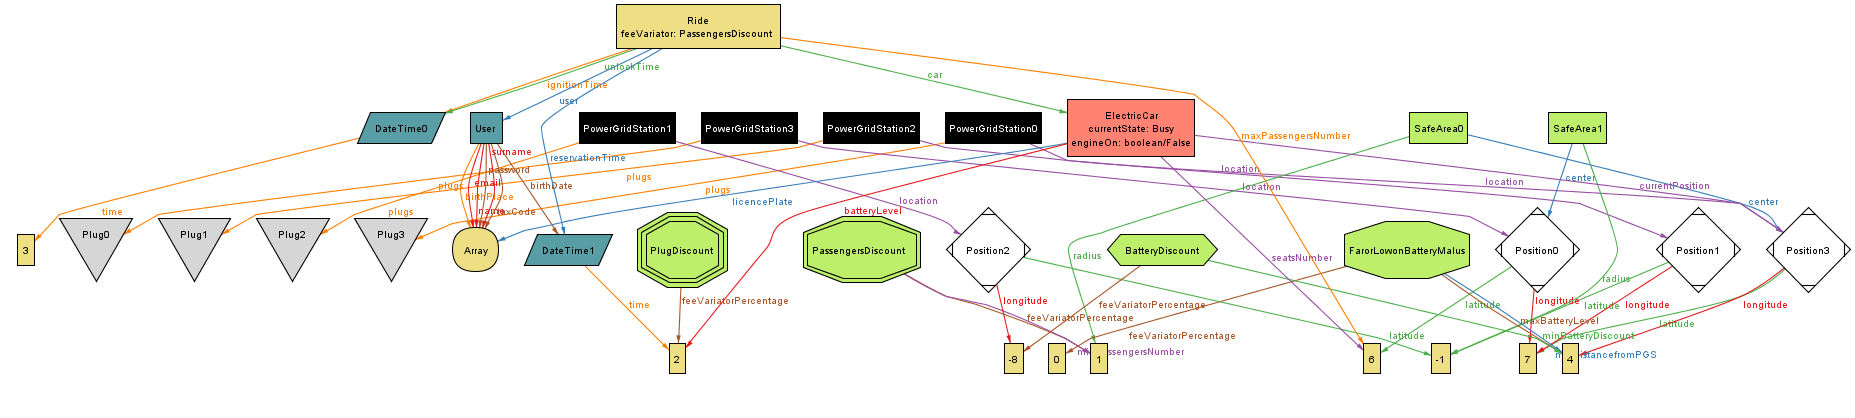
\includegraphics[width=\textwidth]{specific_requirements/alloy/AlloyWorld.png}
    \caption{One possible solution of the Alloy logic model.}
\end{figure}


\chapter{Models}
\section{Class Diagram}
In figure \ref{fig:class_diagram} you can find the class diagram of the system.

\begin{figure}
	\centering
	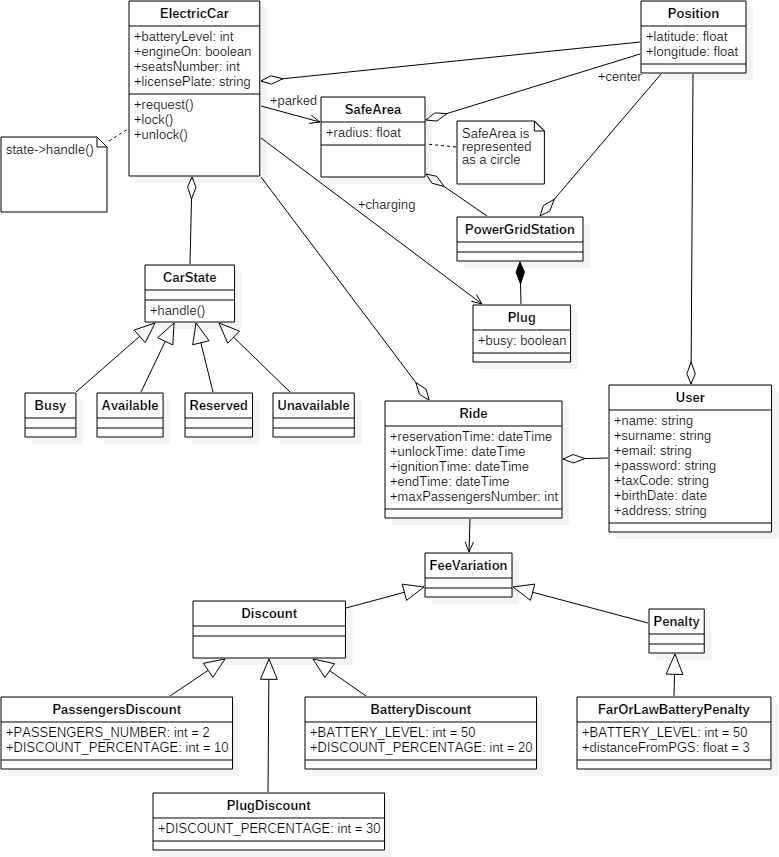
\includegraphics[width=\textwidth,height=\dimexpr\textheight-4\baselineskip-\abovecaptionskip-\belowcaptionskip\relax,keepaspectratio]{uml_models/class_diagram.png}
	\caption{Class diagram of the system.}
	\label{fig:class_diagram}
\end{figure}
\section{Use Case Diagram}
\begin{figure}[p]
\centering
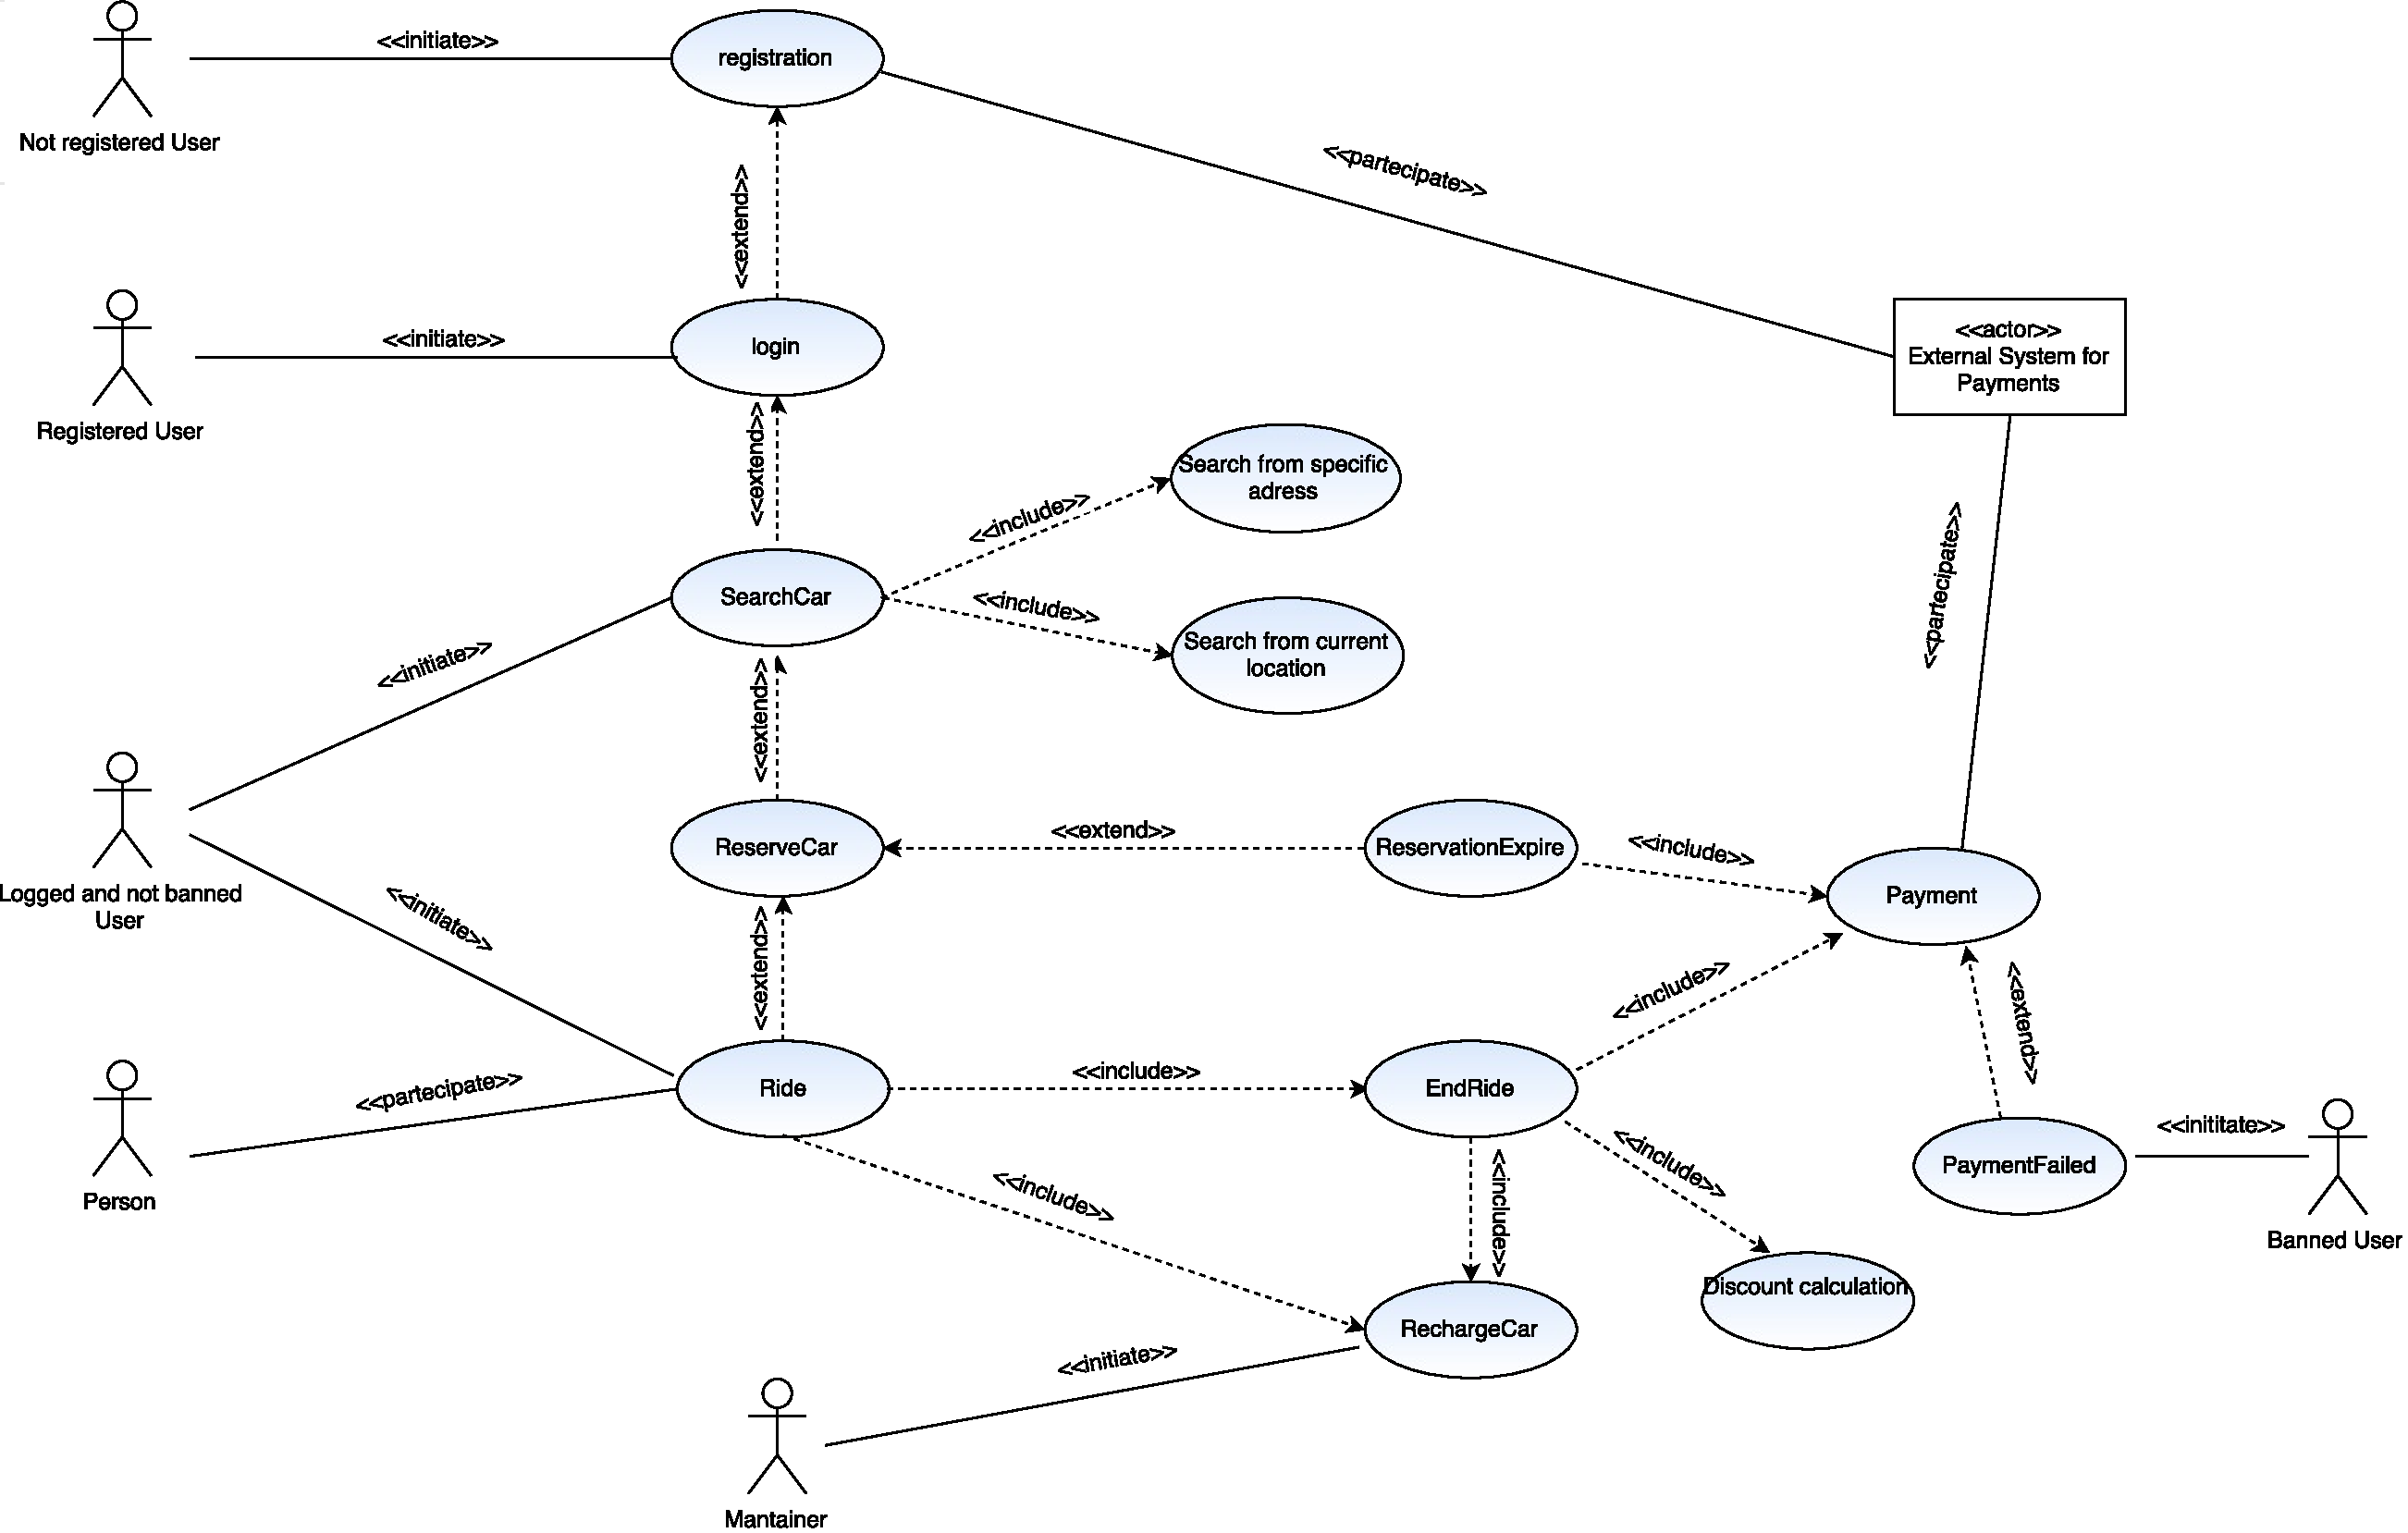
\includegraphics[scale=0.10]{UseCase}
\end{figure}
\section{Use Case Description}
In this paragraph some use cases will be described. These use cases can be derived from the scenarios and the use case diagram.\\
\\
\textbf{User registration} \\
\\
\textbf{Name:}User registration \\
\textbf{Actors:}User,External system for Payments \\
\textbf{Entry conditions:}User is not registered to the system \\
\textbf{Flow of events:} \\
\begin{itemize}
\item The user open the application and click on the button sign up in the homepage;
\item The system show him/her a registration form;
\item The user fill the form with his/her data: name,surname, birth date, driving licence number, credit card number, username and password. Then he/she submit it;
\item The system check the correctness of the data inserted by the user and verify the validity of the credit card through an external system;
\item If all the data are correct the system send him/her a confirmation email of the registration;
\end{itemize}
\textbf{Exit conditions:}The user is successfully registered to the system and now can log in.\\
\textbf{Exceptions:}
\begin{itemize}
\item The information inserted by the user are not valid or some informations are missing.
In this the registration fails and the user is redirected to the homepage.
\item The external system for credit card validation is not available. In this case the user cannot complete the registration until the problem will be fixed.
\end{itemize}


\textbf{User log in} \\
\\
\textbf{Name:} User log in \\
\textbf{Actors:} User \\
\textbf{Entry conditions:} The user is registered to the system and he/she is not banned\\
\textbf{Flow of events:}
\begin{itemize}
\item The user open the application and click on the button log in in the homepage;
\item The system show him a form in which he/she can insert the username and the password;
\item The user fill the form and then click submit it;
\item The system check that the username and password are correct;
\end{itemize}
\textbf{Exit conditions:} The user is successfully logged into the system and now he/she can access to all its functionalities \\
\textbf{Exceptions:} \\
The username and password inserted by the user are not correct.In this case the user is not logged in and he/she will be redirected to the homepage.\\

\textbf{Search Car}\\
\\
\textbf{Name:} Search Car\\
\textbf{Actors:} User\\
\textbf{Entry conditions:} The user is logged into the system \\
\textbf{Flow of events:}
\begin{itemize}
\item The user choose the option "Search Car"
\item The system allows the user to choose one of the 2 options for searching the car: "Search in a specific address" or "Search from current location".
\item If the user choose "Search in a specific address" the system will ask him/her to insert the address and then it will verify the correctness of the inserted data;
\item If the user choose "Search from current location" the system will detect his/her position through the GPS and it will search for car within a range of 1 km from the user's position.
\item The system will show on the map the available cars that satisfy the parameters,with their number and their current battery.
\end{itemize}
\textbf{Exit conditions:} The user can visualize on the map the available cars that fits the parameters \\
\textbf{Exceptions:}  
\begin{itemize}
\item The are no available cars that satisfy the parameters. In this case the user is notified of the unavailability of cars.
\item The address inserted by the user is not correct. In this case the system will ask the user to insert it again
\end{itemize}
\section{BPMN}
todo
\section{Sequence Diagram}
In this paragraph some of the sequence diagram will be described . These diagrams can be derived from the use case descriptions.\\
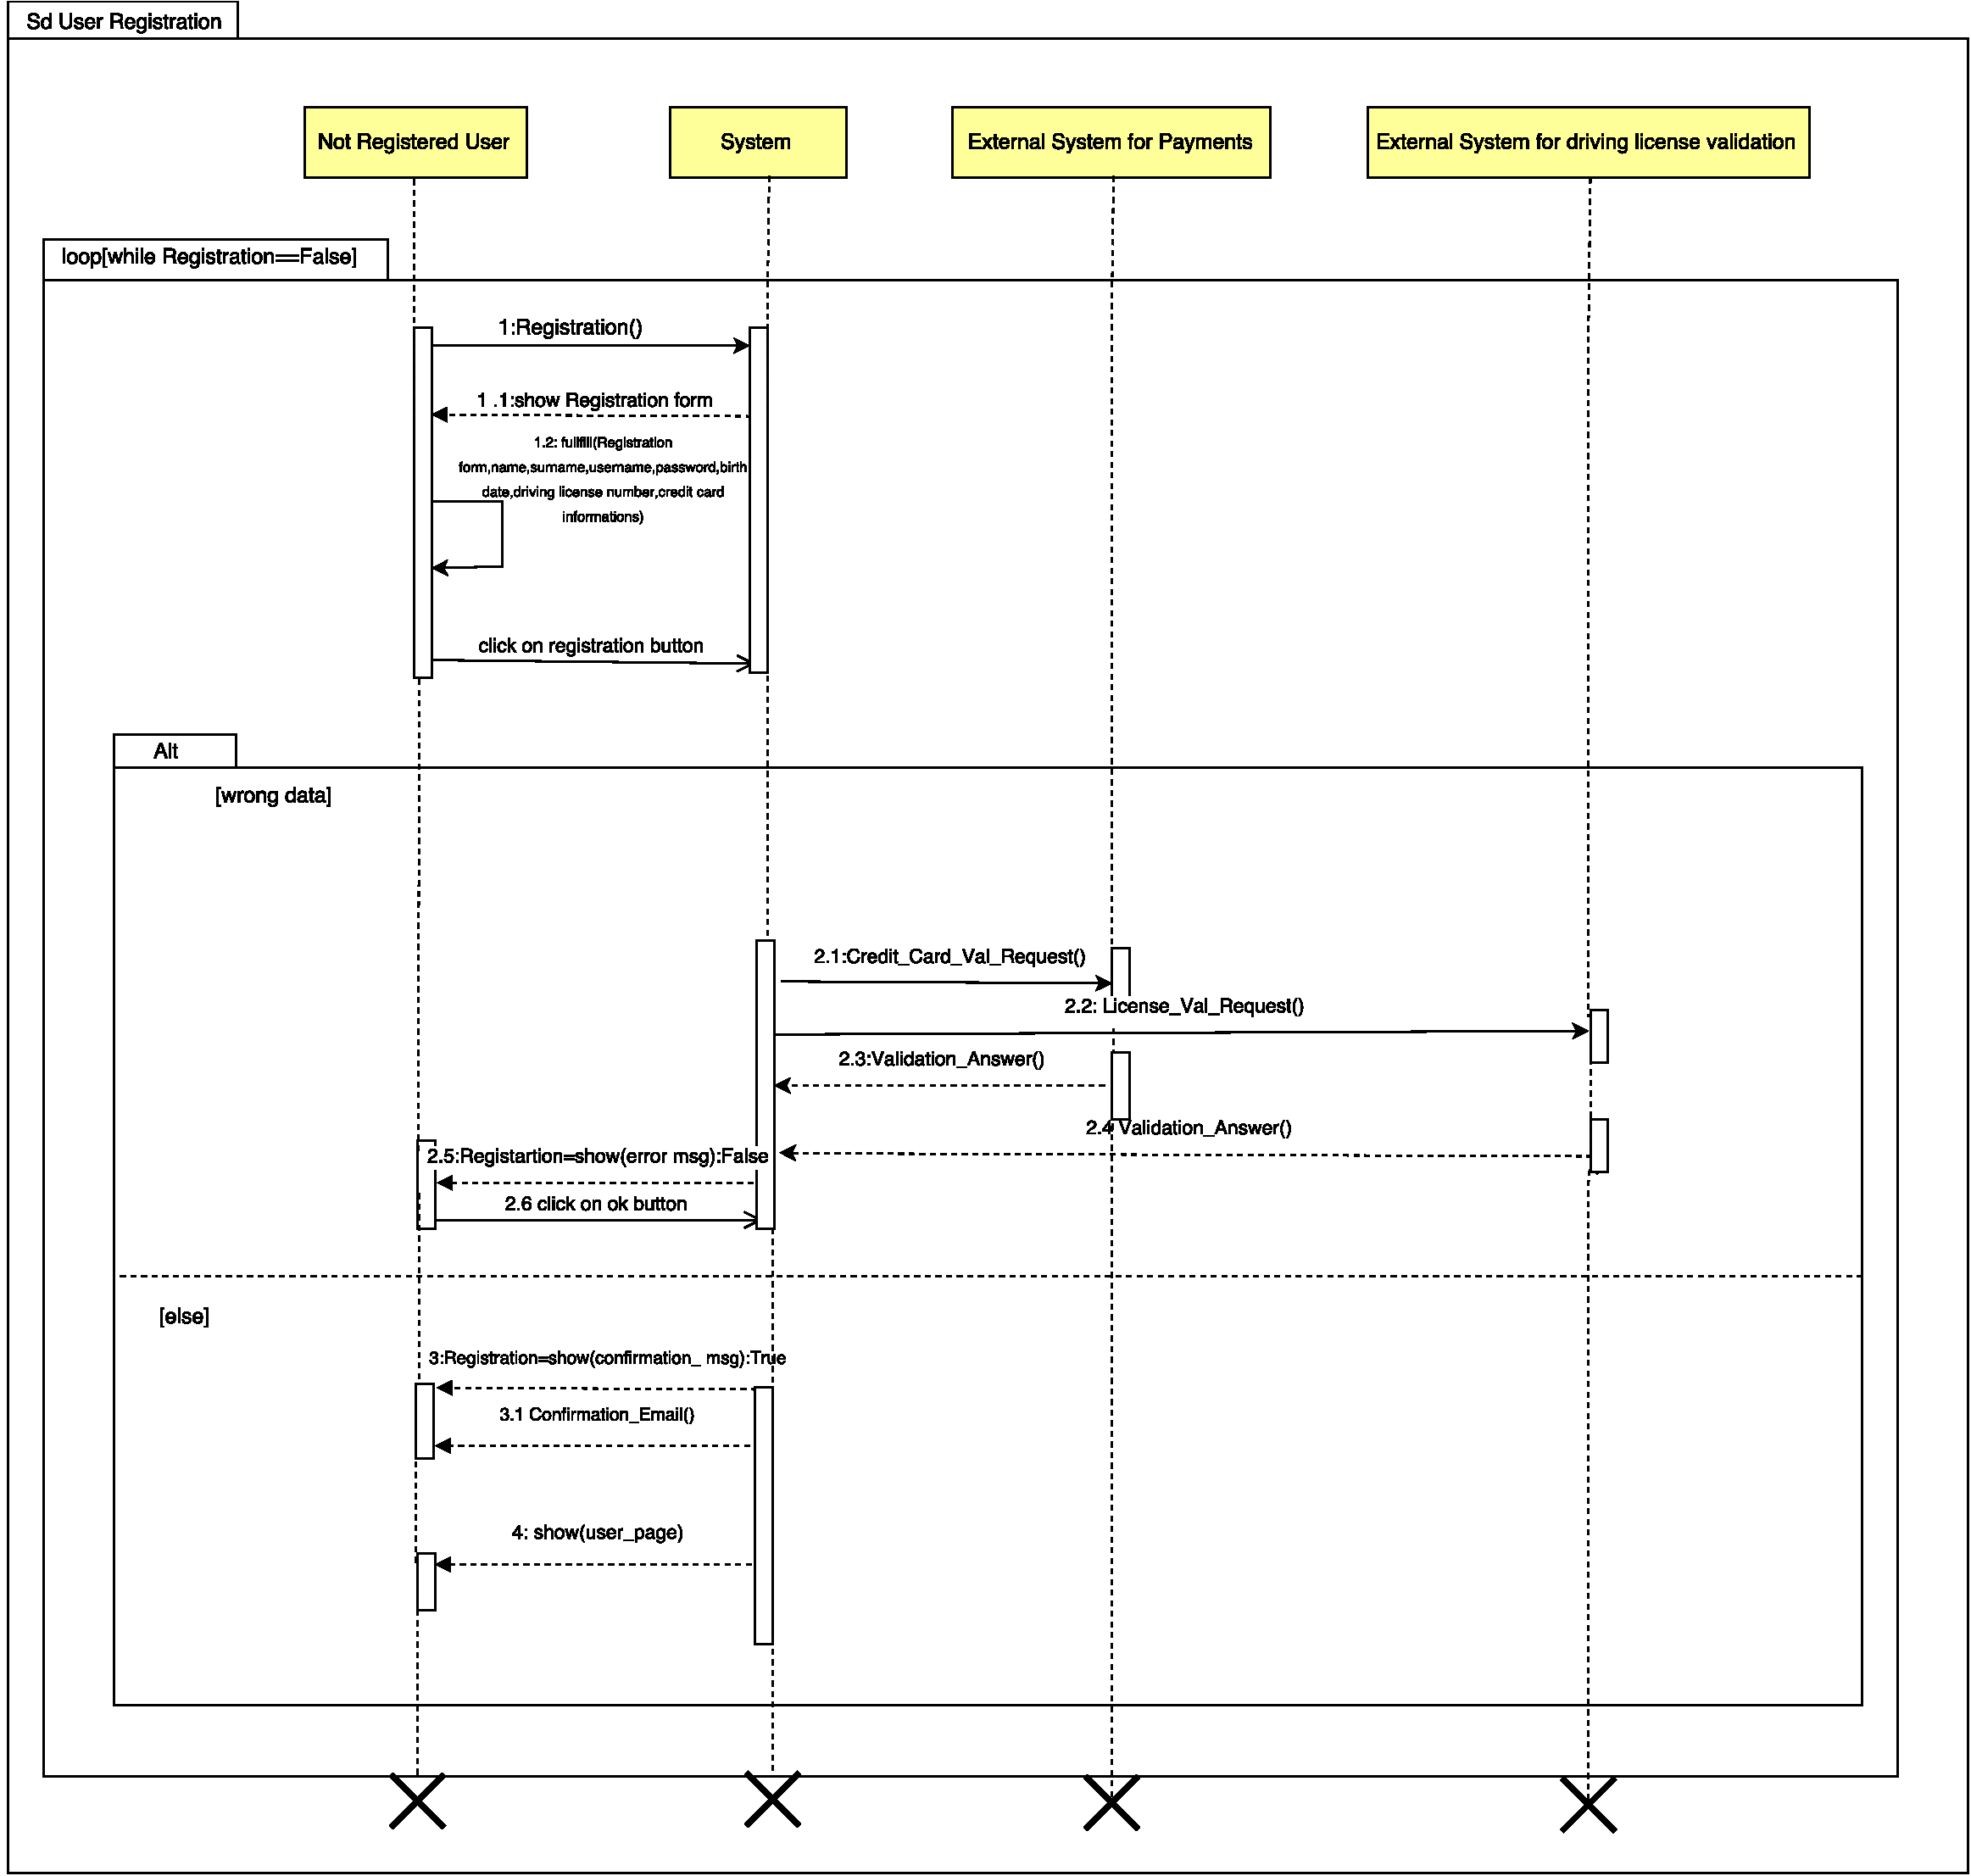
\includepdf{uml_models/RegSeq.pdf}
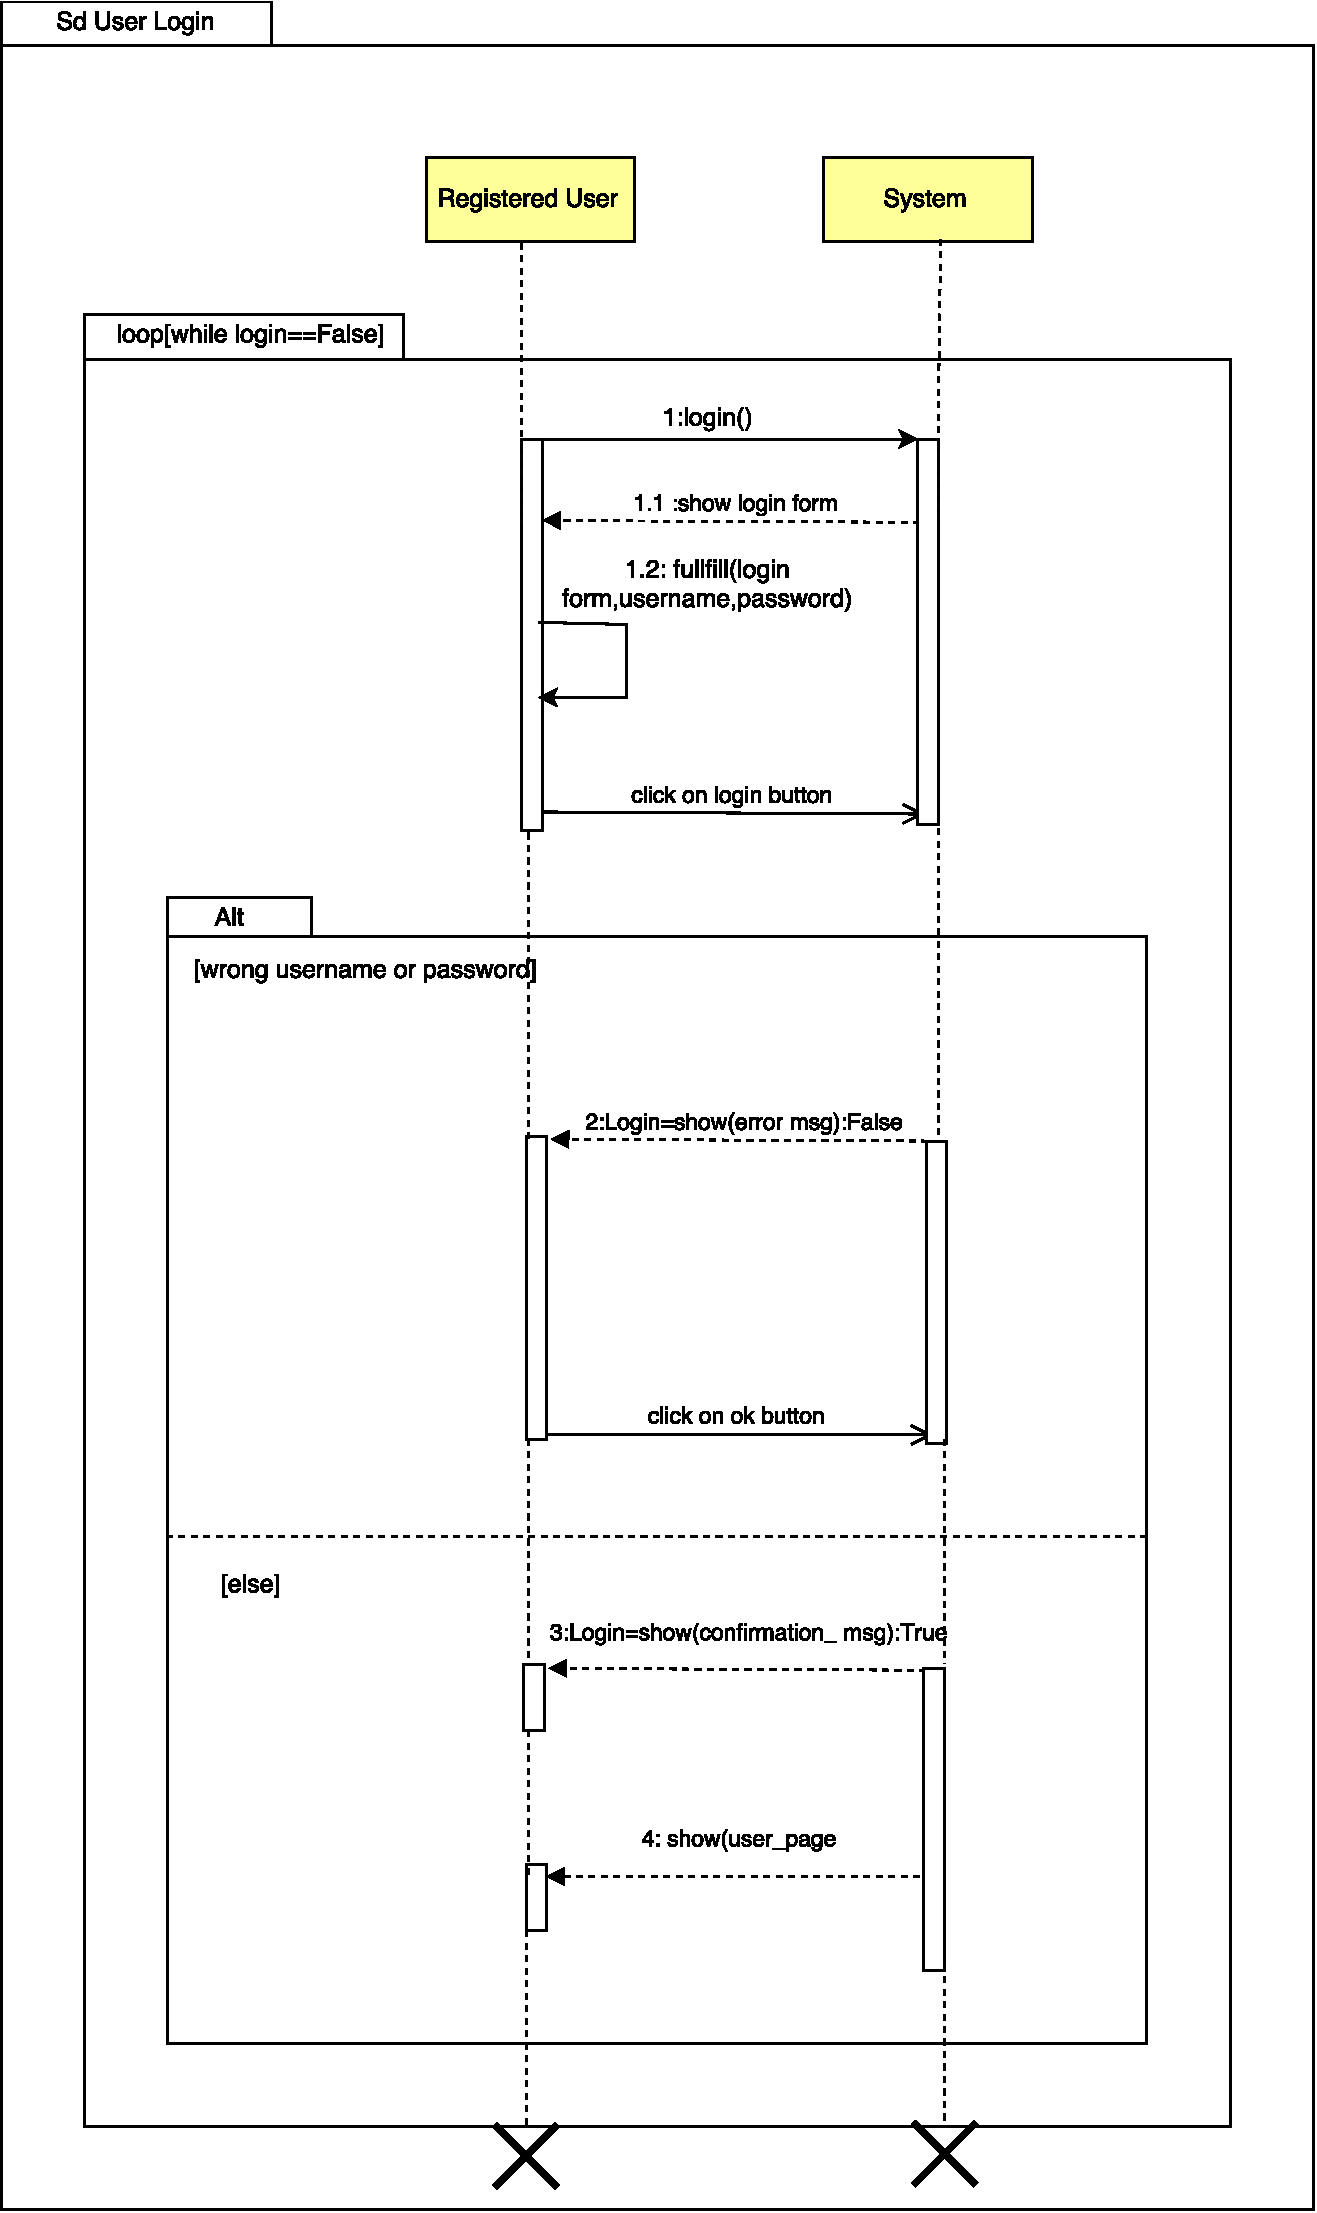
\includepdf{uml_models/LoginSequence.pdf}
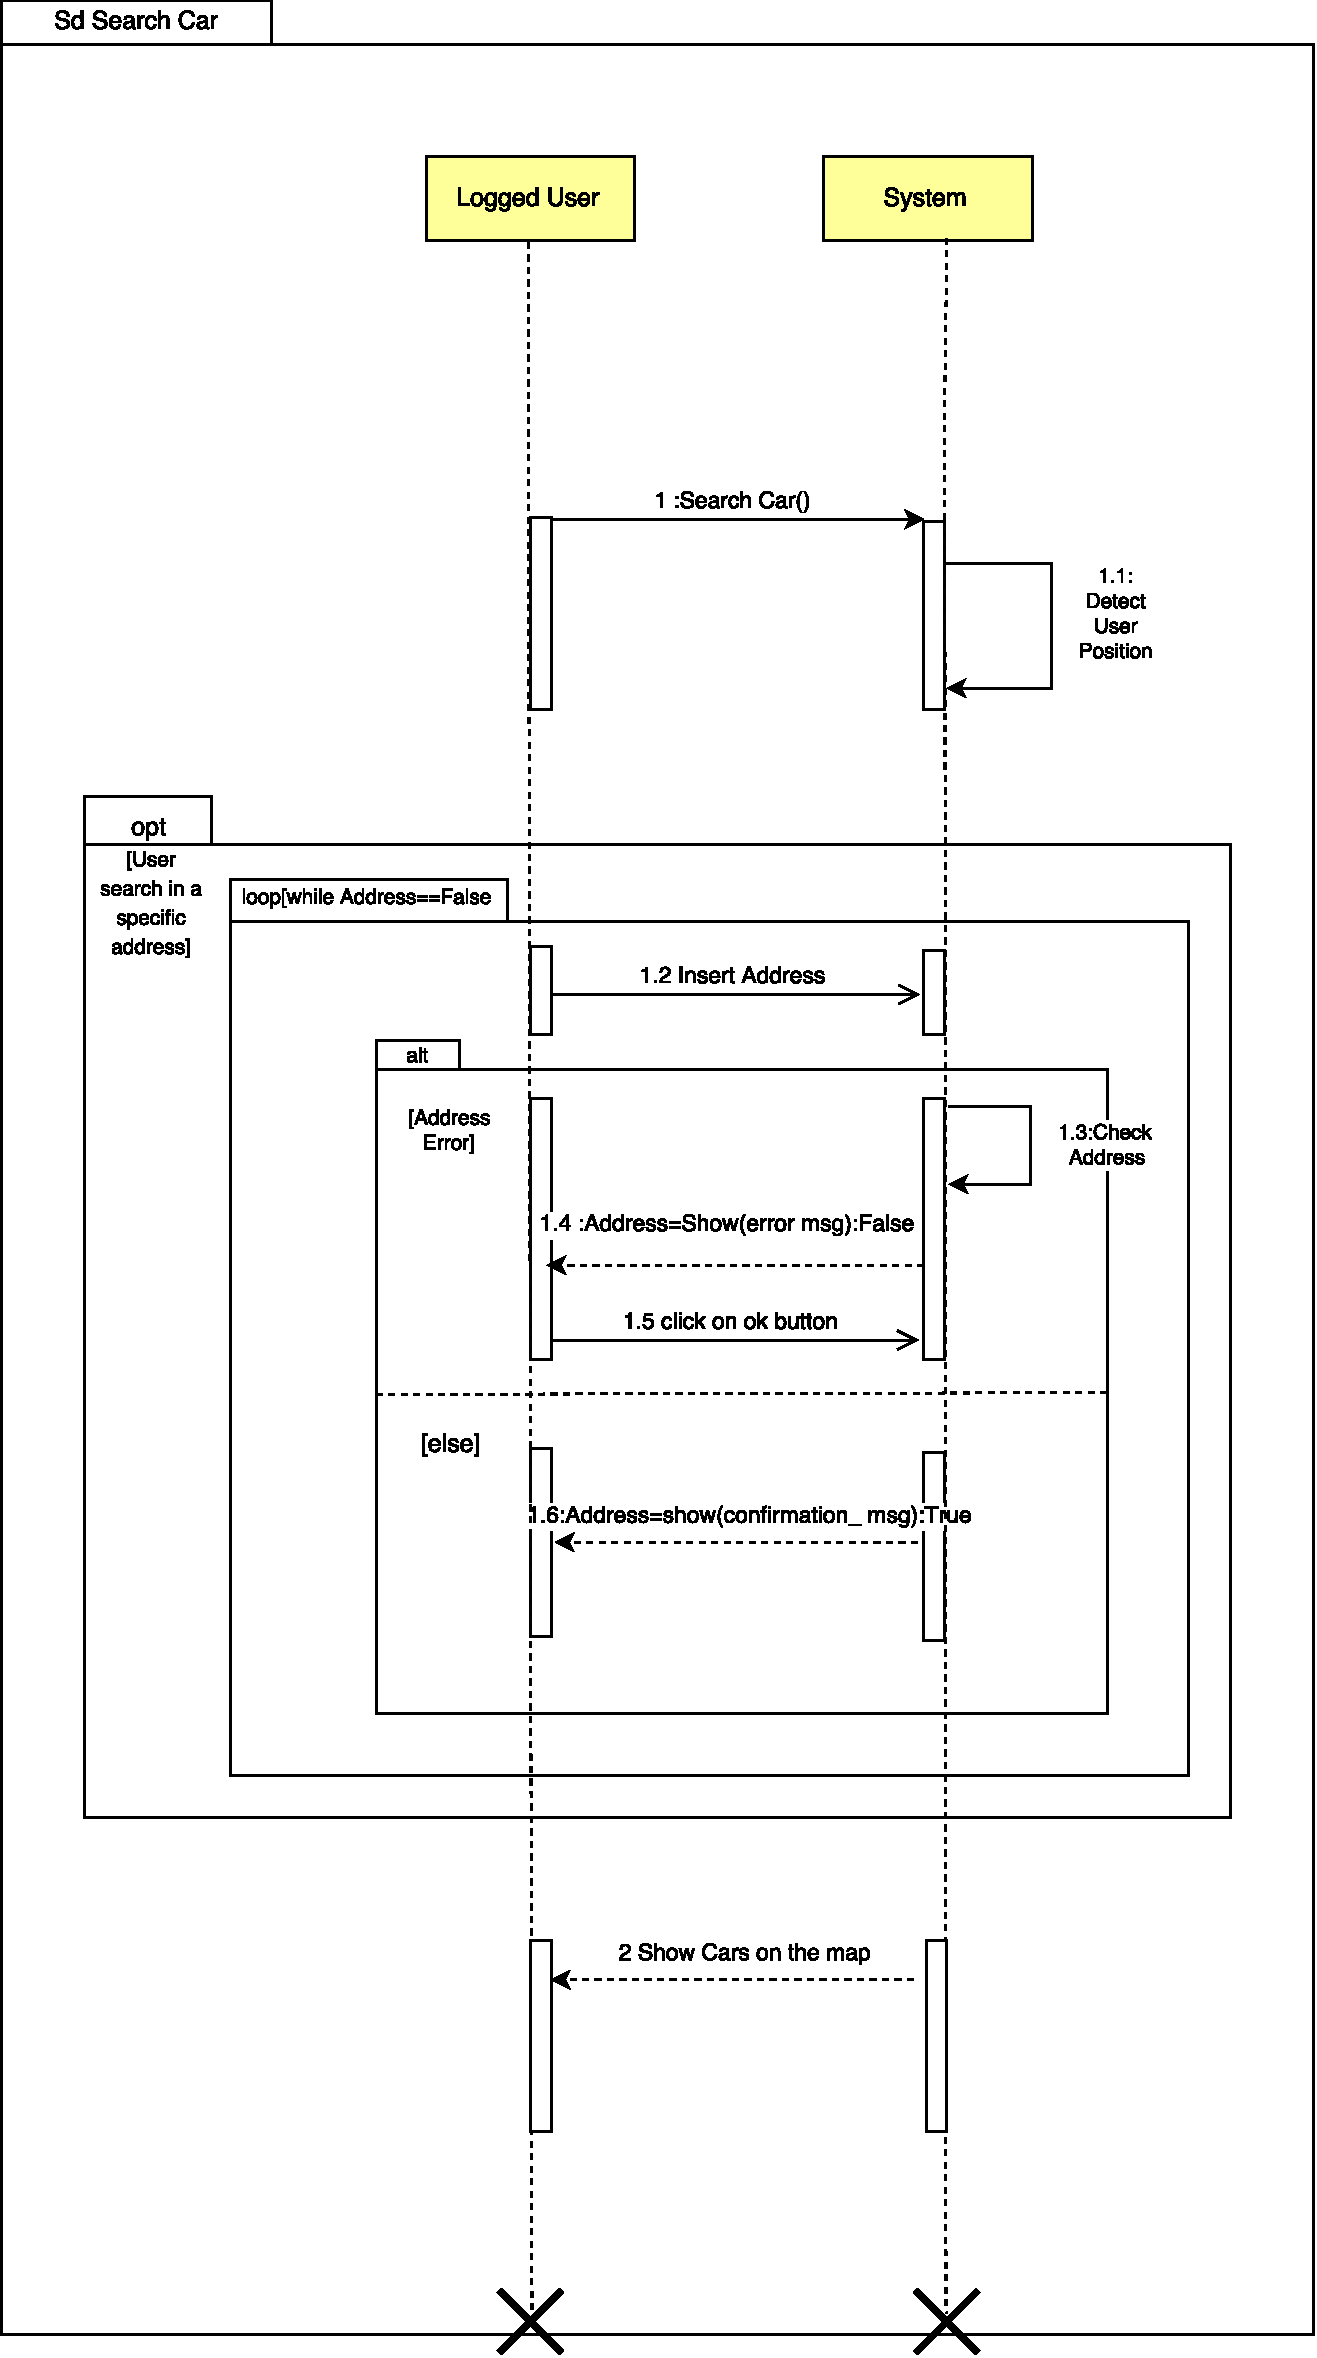
\includepdf{uml_models/SearchCarSeq.pdf}
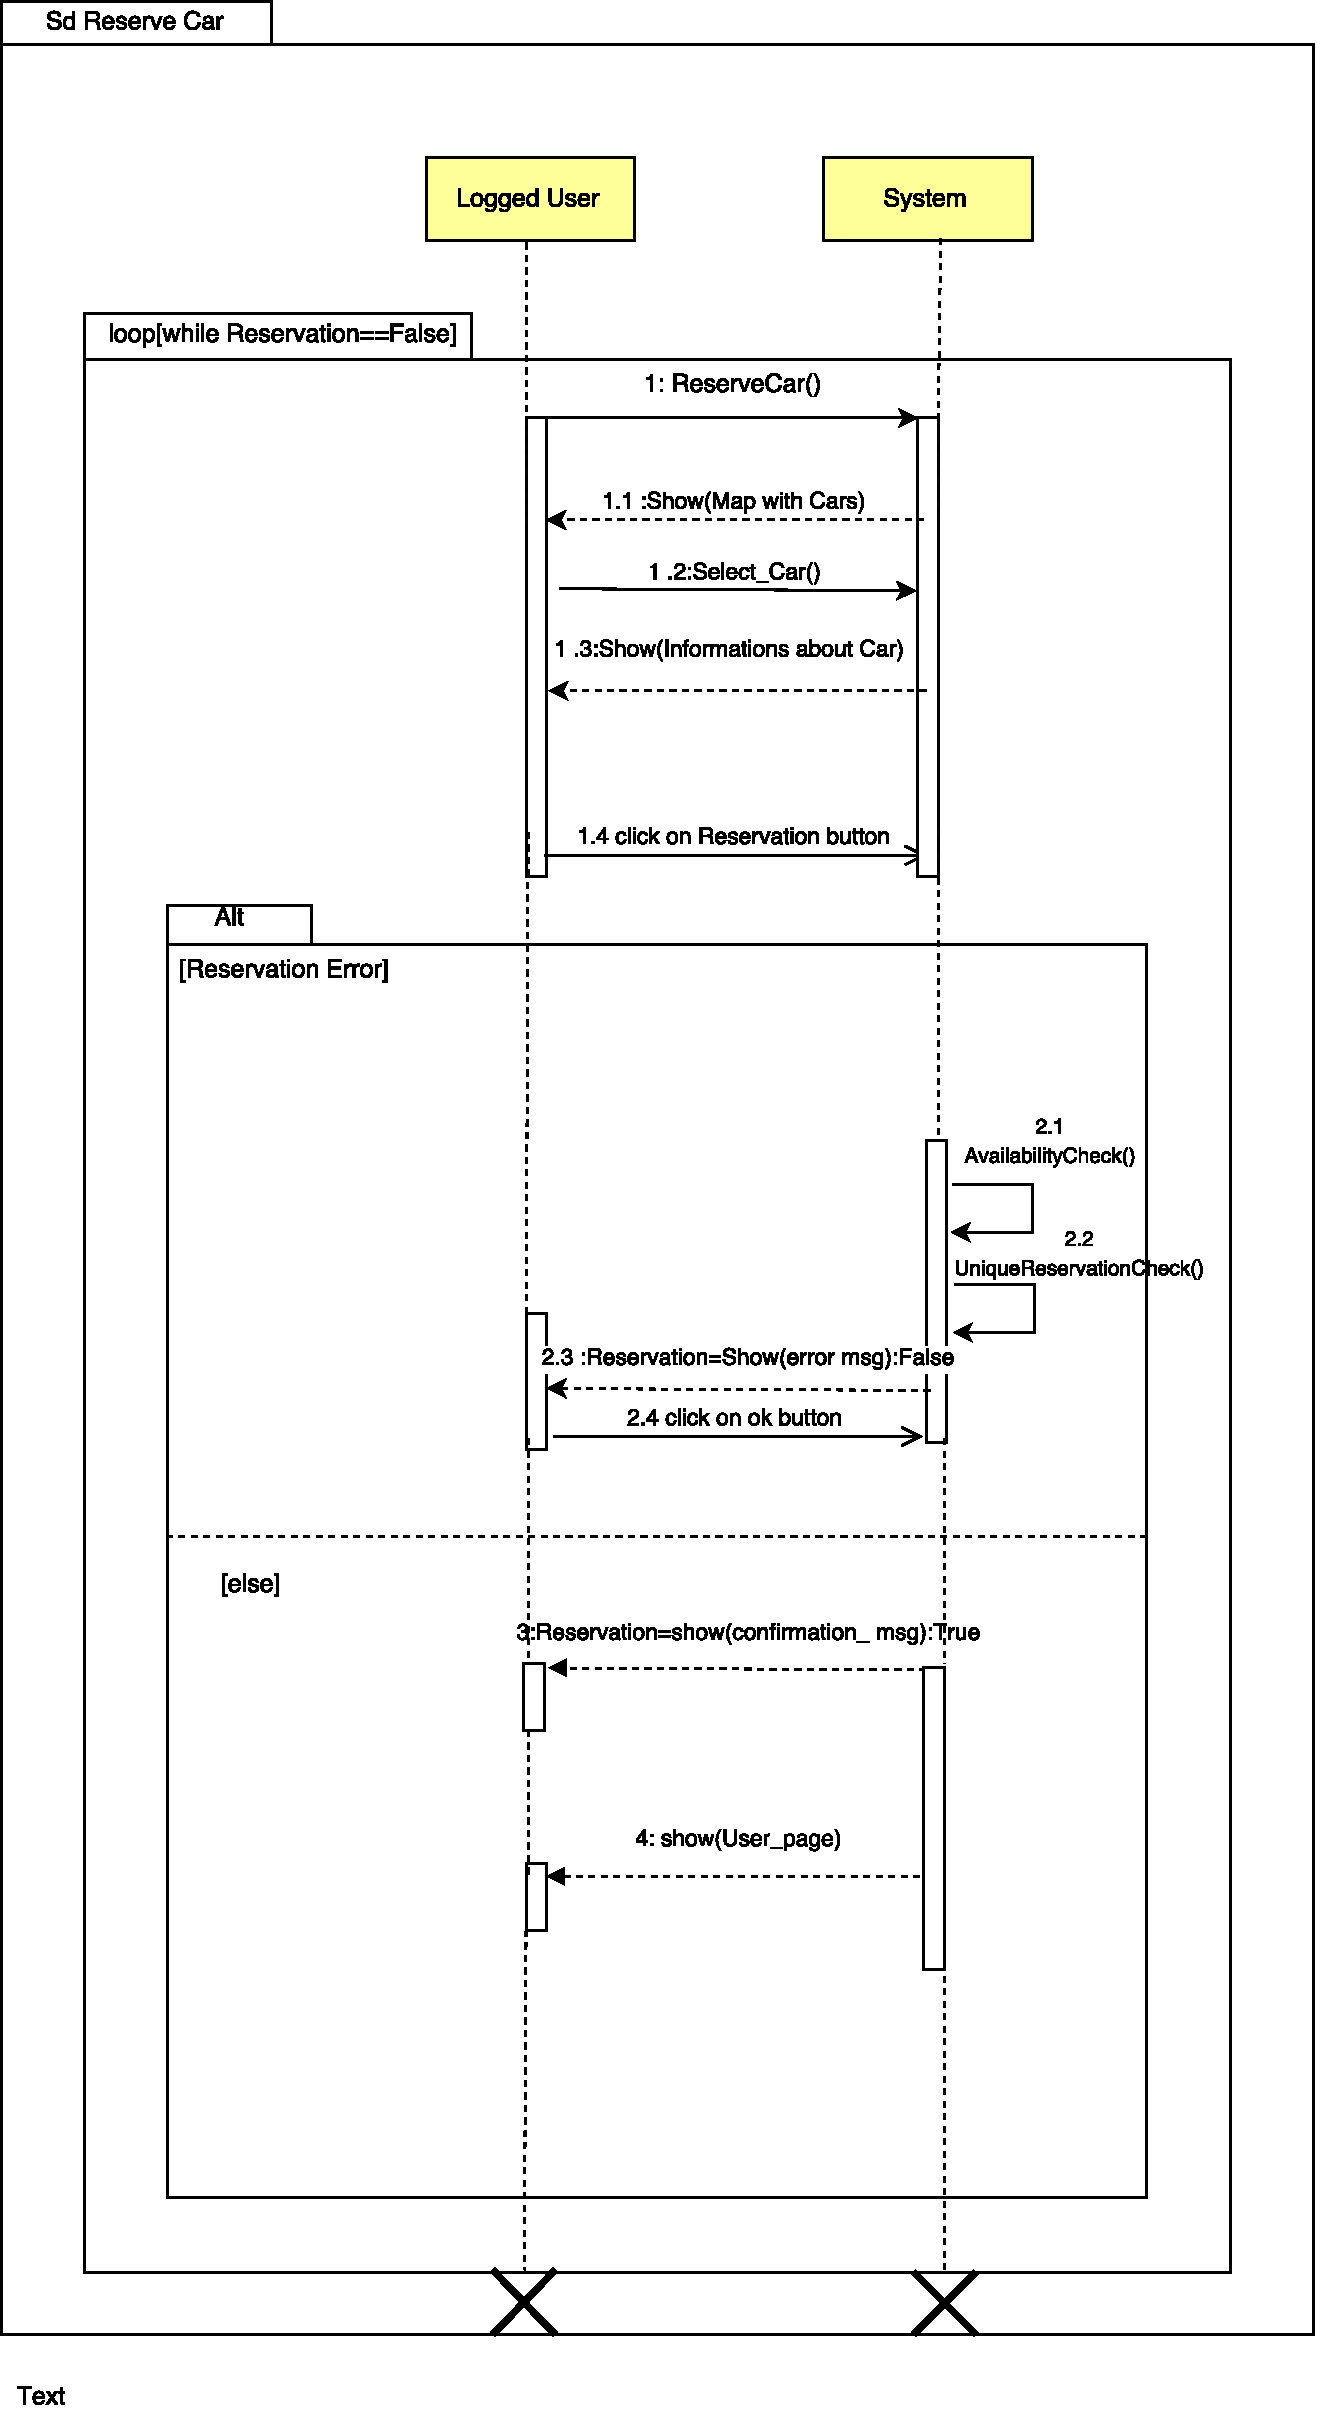
\includepdf{uml_models/ReservationSequence.pdf}
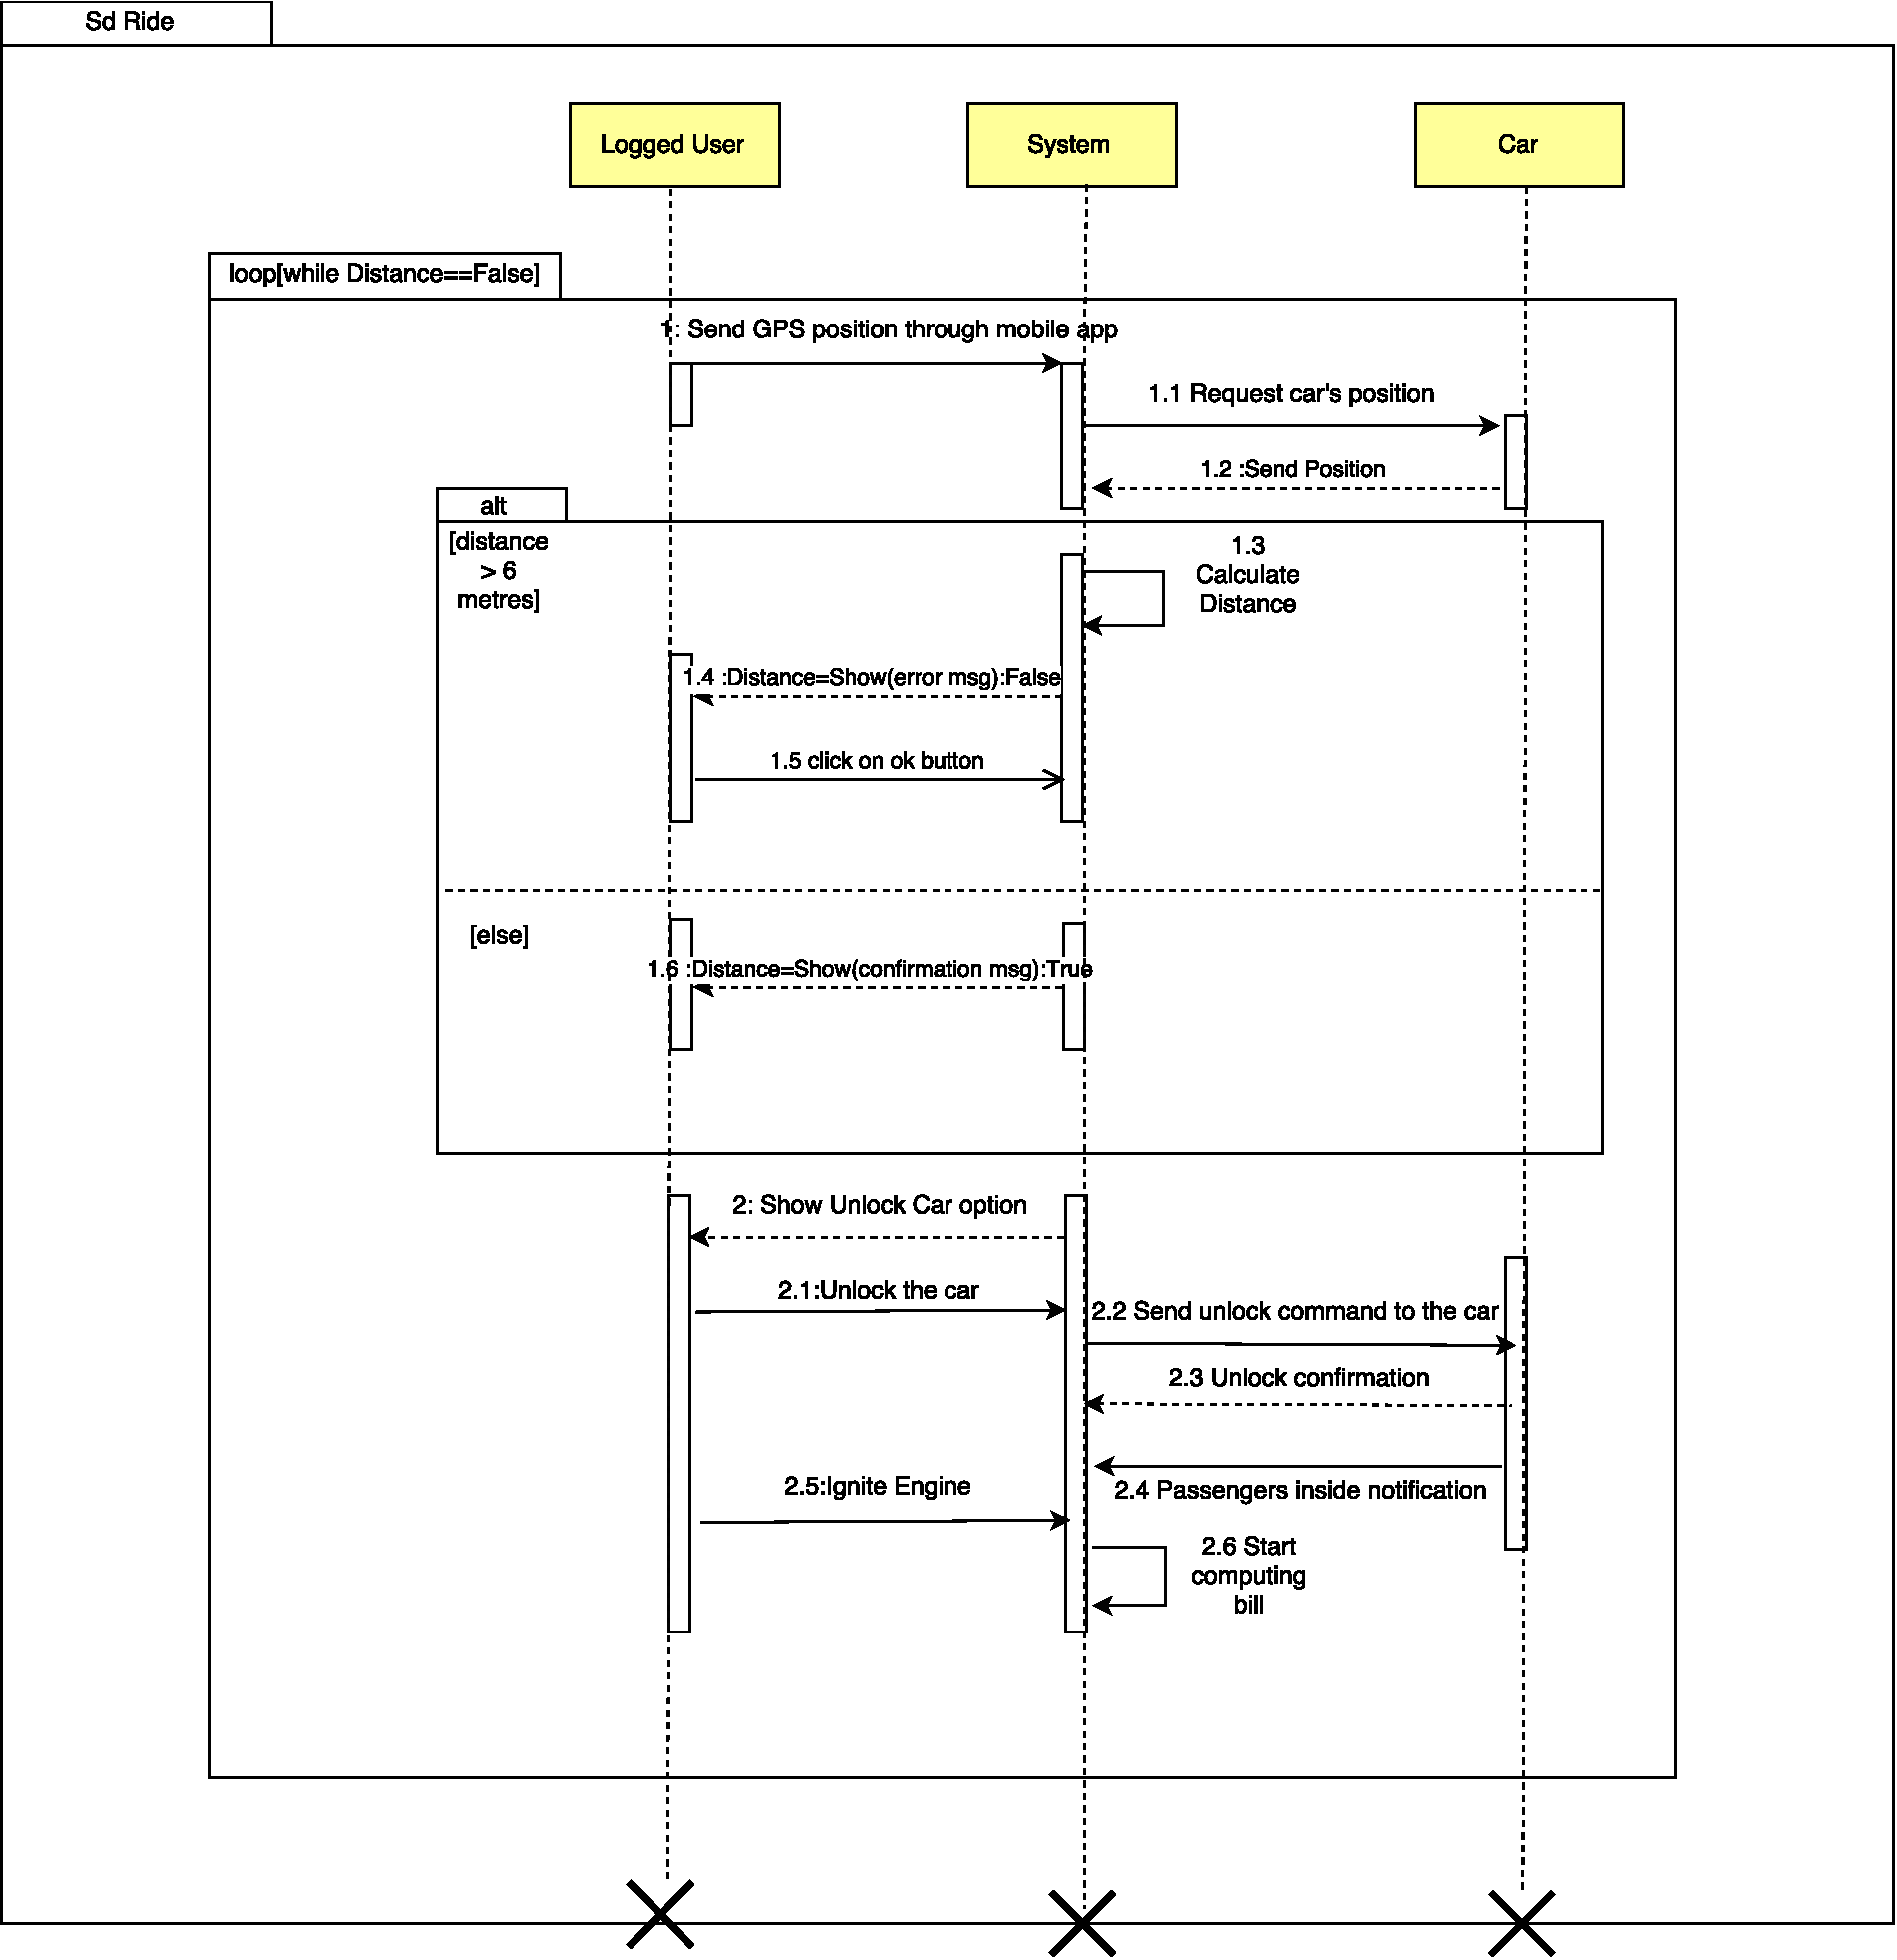
\includepdf{uml_models/RideSequence.pdf}
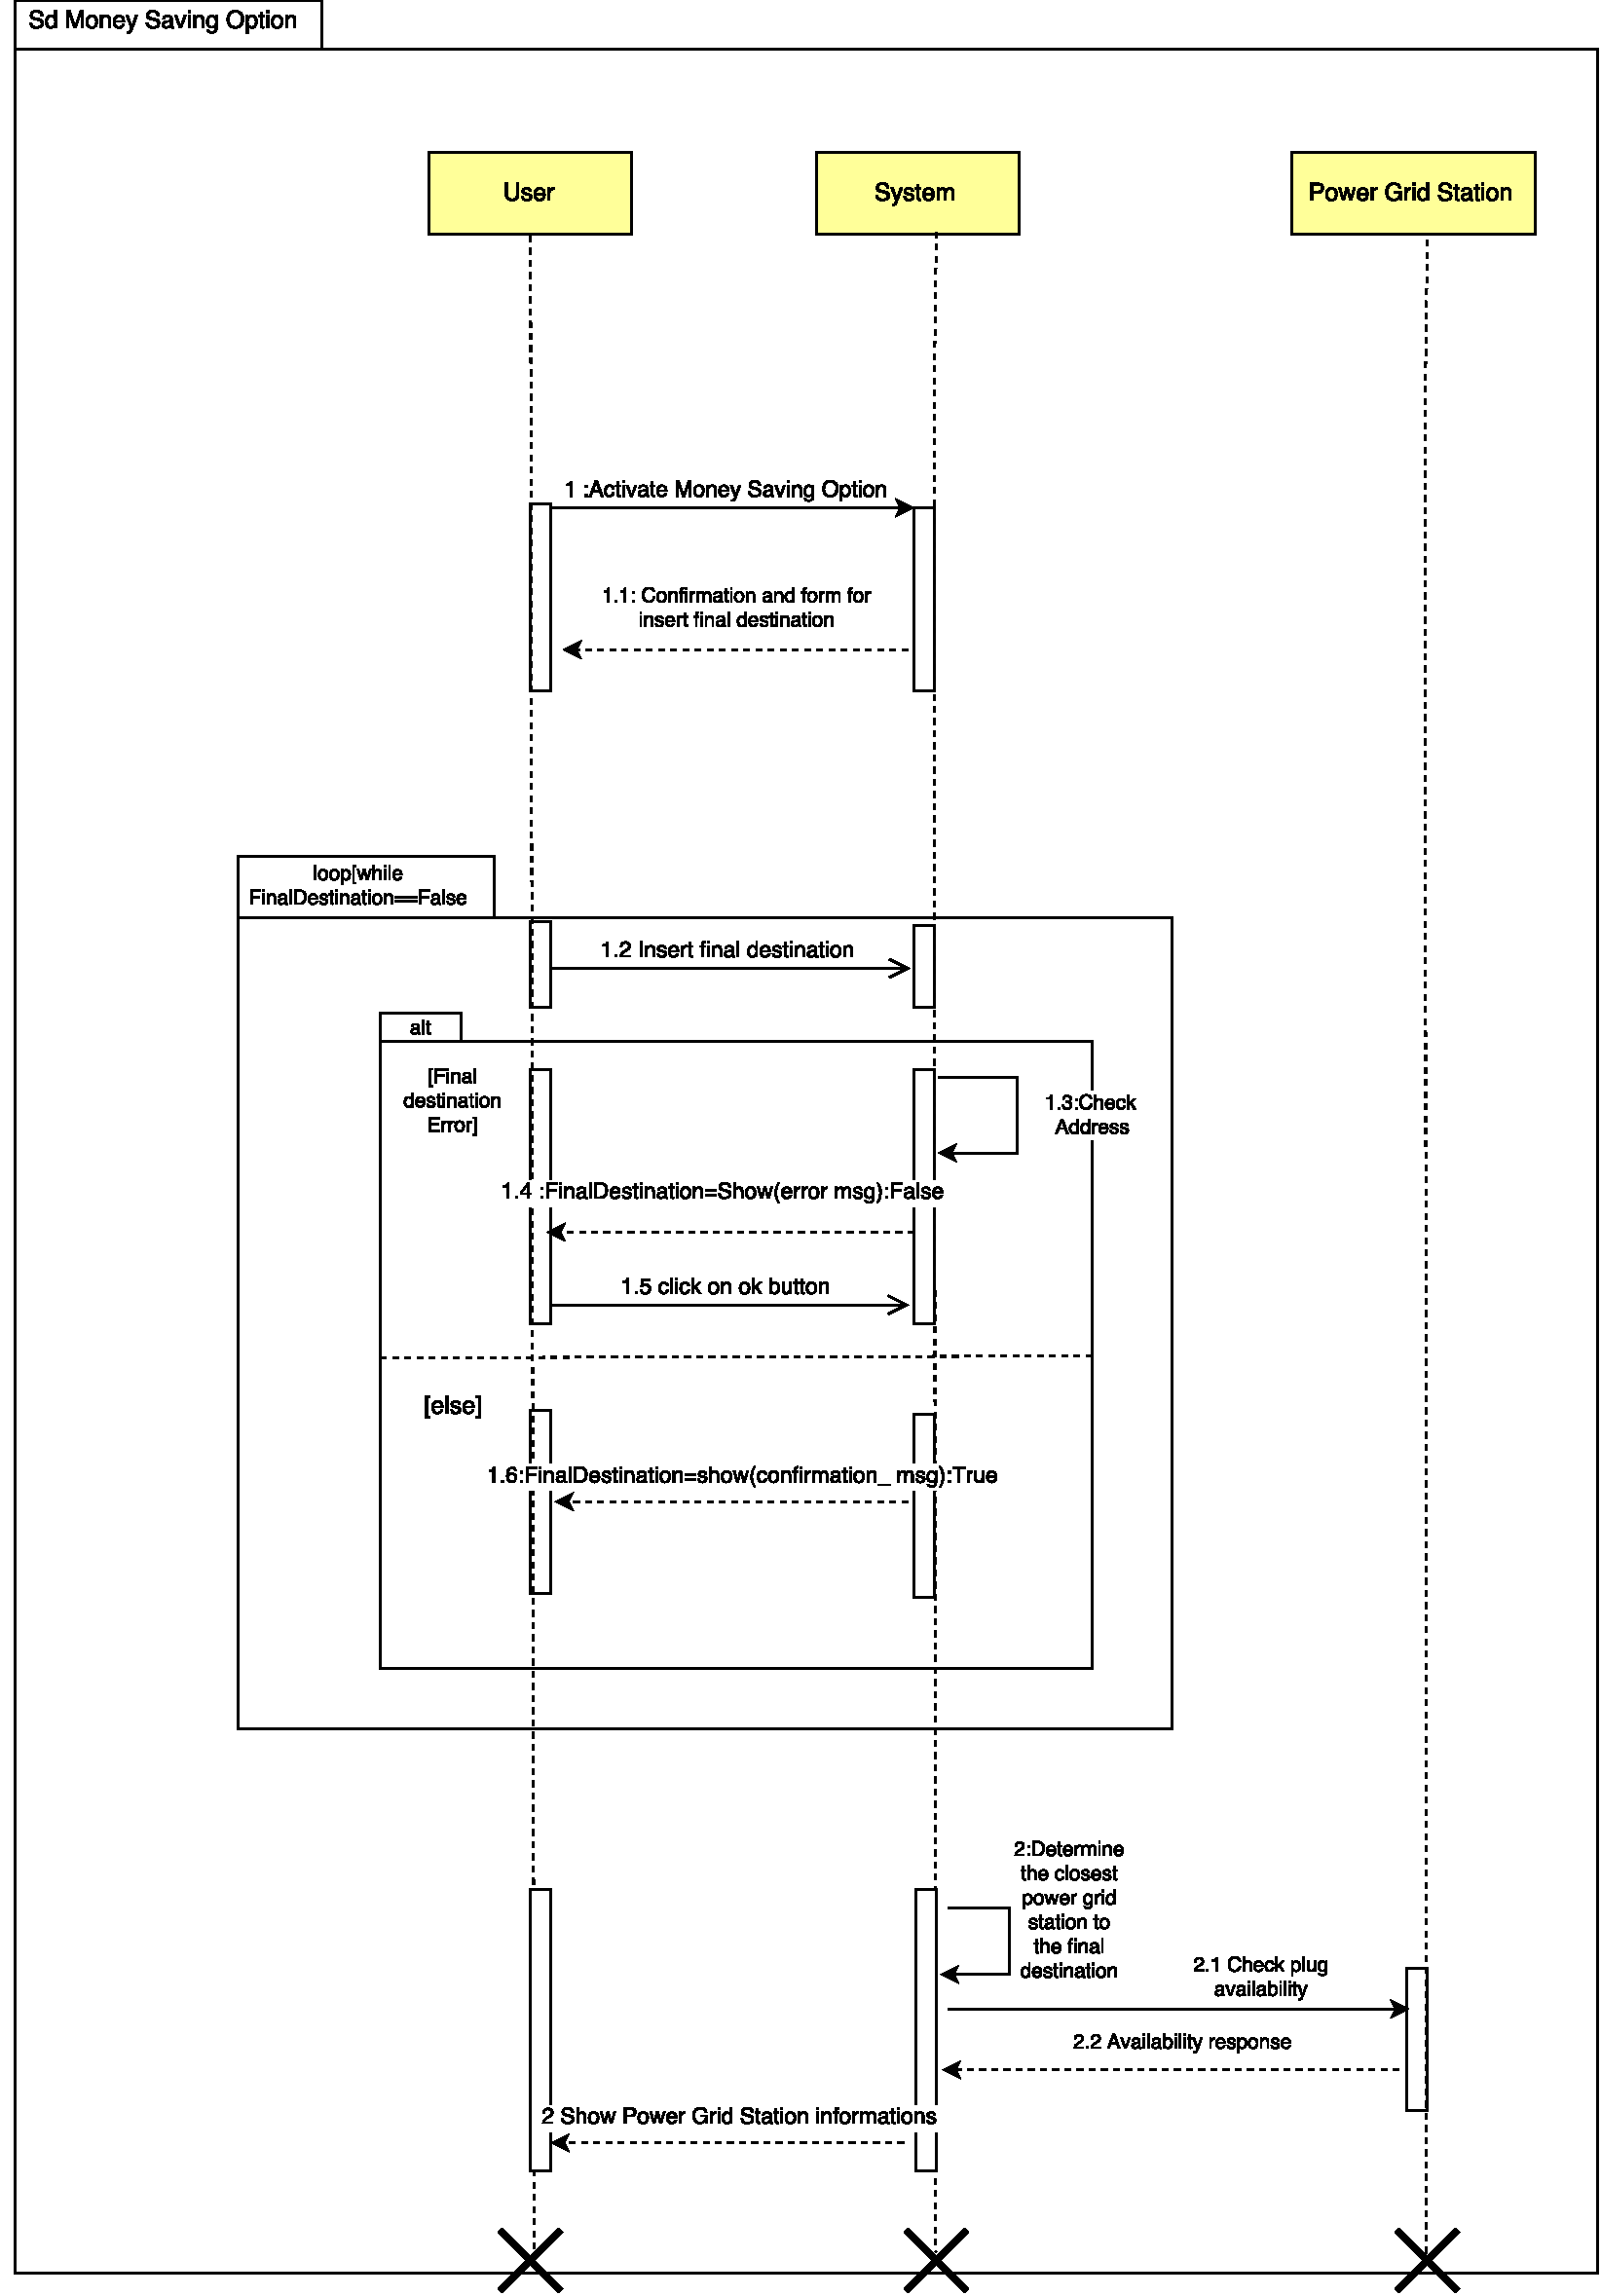
\includepdf{uml_models/SavingMoneySequence.pdf}

\appendix
\chapter{Appendix}
\section{Used software and tools}
\begin{itemize}
    \item \LaTeX\ \footnote{\url{https://www.latex-project.org/}}, for typesetting this document.
    \item Texmaker\footnote{\url{http://www.xm1math.net/texmaker/}}, for the writing of this document.
    \item GitHub\footnote{\url{https://github.com/}} for version control and distributed work.
    \item Evolus Pencil\footnote{\url{http://pencil.evolus.vn/}} for the mockups.
    \item StarUML\footnote{\url{http://staruml.io/}} for the class diagram.
    \item Alloy Analyzer\footnote{\url{http://alloy.mit.edu/alloy/}} used to build the model generated by the alloy code.
    \item Signavio Academic\footnote{\url{http://academic.signavio.com/p/login}} for the use case diagram and for BPMN.
    \item GitHub desktop\footnote{\url{https://desktop.github.com/}} used to collaborate in the team and to keep track of the changes. 
\end{itemize}

\section{Changelog}

v1.1:
\begin{itemize}
\item added car status flow chart;
\item corrected typos;
\end{itemize}

v1.0:
\begin{itemize}
\item initial release.
\end{itemize}

\section{Work hours}
The statistics about commits and code contribution are available on the GitHub repository of the project\footnote{\url{https://github.com/marcomiglionico94/Software-Engineering-2-Project}}.
Please keep in mind that some commits are the joined effort of two or all the components of the group. However, when this is the case, it is specified in the description of the commit.

These are our estimation of the work hours spent on this project:
\begin{itemize}
    \item Marco Ieni: 38 hours
    \item Francesco Lamonaca: 40 hours
    \item Marco Miglionico: 36 hours
\end{itemize}


\end{document}
